\def\OPTIONConf{1}%
\newif\iftr\trtrue
\RequirePackage{etex}
\documentclass[9pt]{sigplanconf}
\toappear{}
% \usepackage[T1]{fontenc}
\usepackage{amsmath}
\usepackage{amssymb}
\usepackage{amsthm}
\usepackage{ stmaryrd }
\usepackage{mathpartir}
\usepackage{balance}
\usepackage{stmaryrd}
\usepackage{wasysym}
\usepackage{multicol}
\usepackage{extarrows}

\usepackage[usenames,dvipsnames,svgnames,table]{xcolor}
\definecolor{light-gray}{gray}{0.9}
\usepackage{soul}
\setulcolor{red}
\usepackage{mathpazo}
\usepackage{colortab}
\usepackage[lowtilde]{url}
\usepackage{todonotes}
\usepackage{listings}
\lstset{tabsize=2,
basicstyle=\ttfamily\fontsize{8pt}{1em}\selectfont}
\usepackage{microtype}
\sloppy
\def \TirNameStyle #1{\small\rulename{#1}}
\renewcommand{\MathparLineskip}{\lineskiplimit=.3\baselineskip\lineskip=.3\baselineskip plus .2\baselineskip}

\usepackage{joshuadunfield}
\iftr

\else
	\usepackage{times}
\fi
% \usepackage{newtxtt}
\usepackage{llproof}
\usepackage{rulelinks}
\newtheorem{theorem}{Theorem}
\newtheorem{lemma}[theorem]{Lemma}
\newtheorem{corollary}{Corollary}
\newtheorem{definition}{Definition}
\newenvironment{proof-sketch}{\noindent{\emph{Proof Sketch.}}}{\qed}
\makeatletter

\usepackage[firstpage]{draftwatermark}
\SetWatermarkText{\hspace*{8in}\raisebox{6.5in}{
\includegraphics[scale=0.1]{aec-badge-popl}}}
\SetWatermarkAngle{0}

\renewcommand\topfraction{0.85}
\renewcommand\bottomfraction{0.85}
\renewcommand\textfraction{0.1}
\renewcommand\floatpagefraction{0.85}

\AtBeginDocument{%
 \abovedisplayskip=2pt plus 4pt
 \abovedisplayshortskip=0pt
 \belowdisplayskip=2pt plus 4pt
 \belowdisplayshortskip=0pt
}

\setlength{\floatsep}{10pt}
\setlength{\textfloatsep}{12pt}

\usepackage[compact]{titlesec}
\titlespacing*{\section}{0pt plus 3pt}{4pt plus 3pt}{2pt plus 3pt}
\titlespacing*{\subsection}{0pt plus 3pt}{4pt plus 3pt}{2pt plus 3pt}
\titlespacing*{\subsubsection}{0pt plus 3pt}{4pt plus 3pt}{2pt plus 3pt}
\titlespacing*{\paragraph}{0pt}{4pt}{3pt}
\setlength{\skip\footins}{3pt plus 1px minus 5px}

% known bug: http://tex.stackexchange.com/questions/1522/pdfendlink-ended-up-in-different-nesting-level-than-pdfstartlink
\usepackage[hidelinks,breaklinks,draft=false]{hyperref}


\usepackage{enumitem}
\makeatletter
\def\thm@space@setup{%
  \thm@preskip=4px plus 2px minus 2px
  \thm@postskip=\thm@preskip % or whatever, if you don't want them to be equal
}
\makeatother

\usepackage{todonotes}
\usepackage{xcolor}

% !TEX root = hazelnut-popl17.tex

% Violet hotdogs; highlight color helps distinguish them
\newcommand{\llparenthesiscolor}{\textcolor{violet}{\llparenthesis}}
\newcommand{\rrparenthesiscolor}{\textcolor{violet}{\rrparenthesis}}

% HTyp and HExp
\newcommand{\hcomplete}[1]{#1~\mathsf{complete}}

% HTyp
\newcommand{\htau}{\dot{\tau}}
\newcommand{\tarr}[2]{#1 \rightarrow #2}
\newcommand{\tnum}{\texttt{num}}
\newcommand{\tehole}{\llparenthesiscolor\rrparenthesiscolor}
\newcommand{\tsum}[2]{{#1} + {#2}}

\newcommand{\tcompat}[2]{#1 \sim #2}
\newcommand{\tincompat}[2]{#1 \nsim #2}

% HExp
\newcommand{\hexp}{\dot{e}}
\newcommand{\hlam}[2]{\lambda #1.#2}
\newcommand{\hap}[2]{#1(#2)}
\newcommand{\hapP}[2]{(#1)~(#2)} % Extra paren around function term
\newcommand{\hnum}[1]{\underline{#1}}
\newcommand{\hadd}[2]{#1 + #2}
\newcommand{\hehole}{\llparenthesiscolor\rrparenthesiscolor}
\newcommand{\hhole}[1]{\llparenthesiscolor#1\rrparenthesiscolor}
\newcommand{\hindet}[1]{\lceil#1\rceil}
\newcommand{\hinj}[2]{\texttt{inj}_{#1}({#2})}
\newcommand{\hcase}[5]{\texttt{case}({#1},{#2}.{#3},{#4}.{#5})}

\newcommand{\hGamma}{\dot{\Gamma}}
\newcommand{\domof}[1]{\text{dom}(#1)}
\newcommand{\hsyn}[3]{#1 \vdash #2 \Rightarrow #3}
\newcommand{\hana}[3]{#1 \vdash #2 \Leftarrow #3}

% ZTyp and ZExp
\newcommand{\zlsel}[1]{{\bowtie}{#1}}
\newcommand{\zrsel}[1]{{#1}{\bowtie}}
\newcommand{\zwsel}[1]{
  \setlength{\fboxsep}{0pt}
  \colorbox{green!10!white!100}{
    \ensuremath{{{\textcolor{Green}{{\hspace{-2px}\triangleright}}}}{#1}{\textcolor{Green}{\triangleleft{\vphantom{\tehole}}}}}}
}

\newcommand{\removeSel}[1]{#1^{\diamond}}

% ZTyp
\newcommand{\ztau}{\hat{\tau}}

% ZExp
\newcommand{\zexp}{\hat{e}}

% Direction
\newcommand{\dParent}{\mathtt{parent}}
\newcommand{\dChildn}[1]{\mathtt{child}~\mathtt{{#1}}}
\newcommand{\dChildnm}[1]{\mathtt{child}~{#1}}

% Action
\newcommand{\aMove}[1]{\mathtt{move}~#1}
	\newcommand{\zrightmost}[1]{\mathsf{rightmost}(#1)}
	\newcommand{\zleftmost}[1]{\mathsf{leftmost}(#1)}
\newcommand{\aSelect}[1]{\mathtt{sel}~#1}
\newcommand{\aDel}{\mathtt{del}}
\newcommand{\aReplace}[1]{\mathtt{replace}~#1}
\newcommand{\aConstruct}[1]{\mathtt{construct}~#1}
\newcommand{\aConstructx}[1]{#1}
\newcommand{\aFinish}{\mathtt{finish}}

\newcommand{\performAna}[5]{#1 \vdash #2 \xlongrightarrow{#4} #5 \Leftarrow #3}
\newcommand{\performAnaI}[5]{#1 \vdash #2 \xlongrightarrow{#4}\hspace{-3px}{}^{*}~ #5 \Leftarrow #3}
\newcommand{\performSyn}[6]{#1 \vdash #2 \Rightarrow #3 \xlongrightarrow{#4} #5 \Rightarrow #6}
\newcommand{\performSynI}[6]{#1 \vdash #2 \Rightarrow #3 \xlongrightarrow{#4}\hspace{-3px}{}^{*}~ #5 \Rightarrow #6}
\newcommand{\performTyp}[3]{#1 \xlongrightarrow{#2} #3}
\newcommand{\performTypI}[3]{#1 \xlongrightarrow{#2}\hspace{-3px}{}^{*}~#3}

\newcommand{\performMove}[3]{#1 \xlongrightarrow{#2} #3}
\newcommand{\performDel}[2]{#1 \xlongrightarrow{\aDel} #2}

% Form
\newcommand{\farr}{\mathtt{arrow}}
\newcommand{\fnum}{\mathtt{num}}
\newcommand{\fsum}{\mathtt{sum}}

\newcommand{\fasc}{\mathtt{asc}}
\newcommand{\fvar}[1]{\mathtt{var}~#1}
\newcommand{\flam}[1]{\mathtt{lam}~#1}
\newcommand{\fap}{\mathtt{ap}}
% \newcommand{\farg}{\mathtt{arg}}
\newcommand{\fnumlit}[1]{\mathtt{lit}~#1}
\newcommand{\fplus}{\mathtt{plus}}
\newcommand{\fhole}{\mathtt{hole}}
\newcommand{\fnehole}{\mathtt{nehole}}

\newcommand{\finj}[1]{\mathtt{inj}~#1}
\newcommand{\fcase}[2]{\mathtt{case}~#1~#2}

% Talk about formal rules in example
\newcommand{\refrule}[1]{\textrm{Rule~(#1)}}

\newcommand{\herase}[1]{\left|#1\right|_\textsf{erase}}

\newcommand{\arrmatch}[2]{#1 \blacktriangleright_{\rightarrow} #2}


\newcommand{\TABperformAna}[5]{#1 \vdash & #2                & \xlongrightarrow{#4} & #5 & \Leftarrow #3}
\newcommand{\TABperformSyn}[6]{#1 \vdash & #2 \Rightarrow #3 & \xlongrightarrow{#4} & #5 \Rightarrow #6}
\newcommand{\TABperformTyp}[3]{& #1 & \xlongrightarrow{#2} & #3}

\newcommand{\TABperformMove}[3]{#1 & \xlongrightarrow{#2} & #3}
\newcommand{\TABperformDel}[2]{#1 \xlongrightarrow{\aDel} #2}

\newcommand{\sumhasmatched}[2]{#1 \mathrel{\textcolor{black}{\blacktriangleright_{+}}} #2}

\newcommand{\subminsyn}[1]{\mathsf{submin}_{\Rightarrow}(#1)}
\newcommand{\subminana}[1]{\mathsf{submin}_{\Leftarrow}(#1)}

\begin{document}

\conferenceinfo{-}{-}
\copyrightyear{-}
\copyrightdata{[to be supplied]}

\preprintfooter{Draft}   % 'preprint' option specified.

\title{Hazelnut: A Bidirectionally Typed \\ Structure Editor
 Calculus}
\subtitle{(Extended Version)}
\authorinfo{
        Cyrus Omar$^1$
        \and Ian Voysey$^1$
        \and Michael Hilton$^2$
        \and Jonathan Aldrich$^1$
        \and Matthew A. Hammer$^3$
}
{
 \begin{tabular}{ccc}
 	\begin{tabular}{c}
 $^1$Carnegie Mellon University, USA\\
 \textsf{\hphantom{$^1$}\{comar, iev, aldrich\}@cs.cmu.edu}
 \end{tabular} &
 \begin{tabular}{c}
 $^2$Oregon State University, USA\\
 \textsf{\hphantom{$^1$}hiltonm@eecs.oregonstate.edu}
 \end{tabular} &
  \begin{tabular}{c}
 $^3$University of Colorado Boulder, USA\\
 \textsf{\hphantom{$^1$}matthew.hammer@colorado.edu}
 \end{tabular}
 \end{tabular}
}
{
 % \vspace{-12px}
}

\maketitle
\begin{abstract}

\emph{Structure editors} allow programmers to edit the tree structure of
a program directly. This can have cognitive benefits, particularly for
novice and end-user programmers. It also simplifies matters for tool
designers, because they do not need to contend with malformed program text.

This paper introduces Hazelnut, a {structure editor} based on a small
bidirectionally typed lambda calculus extended with \emph{holes} and
a \emph{cursor}. Hazelnut goes one step beyond
syntactic well-formedness: its {edit actions} operate over statically
meaningful incomplete terms.  Na\"ively, this would force the programmer to construct terms in a
rigid ``outside-in'' manner. To avoid this problem, the {action semantics}
automatically places terms assigned a type that is inconsistent with the
expected type \emph{inside} a {hole}. This meaningfully defers the type consistency
check until the term inside the hole is \emph{finished}.

Hazelnut is not intended as an end-user tool itself. Instead, it serves as a foundational account of typed structure
editing. To that end, we describe how
Hazelnut's rich metatheory, which we have mechanized using the Agda proof assistant, serves as a guide when we extend the calculus to include binary sum types. We also discuss various interpretations of holes, and in so doing
reveal connections with gradual typing and contextual modal type theory, the Curry-Howard interpretation of contextual modal logic. Finally, we
discuss how Hazelnut's semantics lends itself to implementation as an event-based functional reactive program. Our simple reference implementation is written using \lstinline{js_of_ocaml}.

\end{abstract}

\category{D.3.1}{Programming Languages}{Formal Definitions and Theory}
\category{D.2.3}{Software Engineering}{Coding Tools and Techniques}[Program Editors]
%\category{F.3.1}{Logics \& Meanings of Programs}{Specifying and Verifying and Reasoning about Programs}[Specification Techniques]
\keywords
structure editors, bidirectional type systems, gradual typing, mechanized metatheory

\section{Introduction}\label{sec:introduction}
% !TEX root = hazelnut-popl17.tex

%% Programs (and, by the Curry-Howard correspondence, proofs) are rich
%% inductive structures. This fact is well understood amongst researchers
%% and experienced programmers, but still somewhat obscure amongst
%% programmers at large because programmers normally construct and interact
%% with programs only indirectly, e.g. using a text editor composed with a
%% parser.

%% There are some benefits to this approach, to be sure, but the structural
%% mismatch between programs and their textual representations also imposes
%% various burdens.  For example, the primitive edit actions available in a
%% text editor (e.g. inserting or deleting a character or word) do not
%% always correspond to sensible structural transformations.

% spj: describe the problem; state our contributions; STOP. one page max.

% When constructing a program or proof in a language with rich type
% structure, skilled programmers generally follow a \emph{type discipline}
% where they first determine the type of the expression that they are
% constructing in order to constrain the mental search space that they are
% operating within.

% For example, if the programmer knows that an expression of type
% $\tarr{\tnum}{\tnum}$ is needed, then it is often the case (though, of course, not
% necessarily the case) that the expression will take the form $$\hlam{\mathit{x}}{e}$$
% for some variable $x$ and function body $e$. If the programmer chooses this
% form, then after picking a suitable variable name, her focus will be on
% constructing a suitable body, $e$. Following the type discipline, $e$ must
% be of type $\tnum$, and so this process can begin anew.

% The problem is that when using a text
% editor to construct a program, it is easy, and indeed necessary, to deviate from this disciplined process.  Rather, text editors operate on sequences of
% characters (i.e. \emph{text}.) 

%Although programs can be represented as text, most text does not correspond to a syntactically well-formed and semantically well-defined program. 
% Programming languages, and therefore programs themselves, are rich mathematical structures. 
Well-typed programs are rich semantic structures, but human programmers typically construct and manipulate them only indirectly: by editing text that is parsed according to a textual syntax and then typechecked according to a static semantics. This indirection is of substantial practical utility, to be sure -- text editors and other text-based tools benefit from decades of development effort. However, it also introduces some fundamental complexity into the programming process. 

% Every day, programmers use text-based tools to construct and manipulate programs.  
% These programs are written in languages which defined by a textual syntax. 
% While textual syntax has proved to have practical utility, it also introduces some fundamental complexity into the programming process.

% It also complicates matters for tool designers because tools are often confronted with text that does not correspond to a well-formed, meaningful program\todo{mention YoungSeok's data here}. This may be because the programmer is in the midst of a sequence of 
% edit actions that leaves the text temporarily malformed or ill-typed, or because the programmer has made a mistake. The language definition is silent about these situations, so it is difficult for tools to help programmers determine and execute a corrective course of action (e.g. by providing \todo{cite study on benefits of syntax highlighting}syntax highlighting and semantics-aware code completion services\todo{cite something?}.)
%Doesn't really start out with a bang, IMHO. I like to start papers out with a "big" problem.
%Most programming languages define a textual syntax. This allows programmers to use text editors and other standard text-based tools to construct and manipulate programs. While this is of substantial practical utility, it also introduces some fundamental complexity into the programming process. 

First, it requires that programmers understand the various subtleties of textual syntax (e.g. the relative precedence of the various forms.) This can be particularly challenging for novice and end-user programmers \cite{Altadmri:2015:MCI:2676723.2677258}. %For example, one study of novice programmers found syntax errors (e.g. unbalanced parentheses) to be the most common class of errors.
% Too much detail? 

Moreover, the fact that not all sequences of characters correspond to a well-formed, meaningful program complicates matters for tool designers. Tools are confronted with such text quite frequently -- by analyzing a dataset gathered by Yoon and Myers \cite{6883030} (which contains 1,460 hours of fine-grained edit logs collected from 21 programmers) we found that 44.2\% of code edits resulted in malformed edit states. Some additional percentage of edit states were well-formed but ill-typed (the dataset did not include enough information to determine the exact percentage.)  
Some of these edit states were due to programmer error, while others arose simply because the programmer was in the midst of a sequence of edit actions that left the text temporarily malformed or ill-typed. The language definition is silent about these edit states, so it is difficult to design useful editor services (e.g. syntax highlighting~\cite{sarkar2015impact} and semantics-aware code completion~\cite{Mooty:2010:CCC:1915084.1916348}) and report meaningful error messages\todo{citations}.
%, or because the programmer has made a mistake. 
% The syntax definition is silent about these situations, so it is difficult for tools to help programmers determine and execute a corrective course of action 

Some editors have developed \emph{ad hoc} workarounds for this problem, e.g. they might attempt to insert closing delimiters automatically, use whitespace to guess where a construct is likely to end, use regular expressions to highlight malformed program text, or recover from a type error by pretending that the type was as expected (if, indeed, an expected type can be determined.\todo{citations?}) These heuristic methods are imperfect, complex and sometimes misleading. % This may also help explain why the error messages emitted by parsers and typecheckers are often quite baroque\todo{citations}.

% stuck editing a representation of the program instead of the structures
% themselves. The editor does not restrict what the programmer may do: you
% can delete characters that belong, insert ones that don't, forget things
% that were needed, and so. There's nothing stopping us from accidentally
% writing $$\lambda \mathit{x:num}.\mathit{(x,x)}$$ even though it's obvious
% that building a pair can't hope to form a natural number.

% The type structure of the language makes this sort of error obvious: it's
% not that you're adding characters that make your program incorrect, or even
% malformed; you're adding characters that can't possibly create a structure
% you want because of the type. Simply put, the primitive operations
% available in text editors do not always correspond to sensible
% transformations on the structure of the program.
One attempt to solve this problem has been \emph{Structure editors},
where every edit action leaves the program being manipulated in a 
structurally well-formed state.\footnote{In addition to eliminating malformed edit states, it is also often promised that programs can be written more quickly using a structure editor. However, we will not discuss such ``edit costs'' here, because they depend on particular implementation details, e.g. whether a keyboard or a mouse is in use.} 
%Scratch etc. for novices. mbeddr for pros. Lamdu and Unison ongoing efforts with a functional foundation. We give other examples of notable structure editors in Sec. \ref{sec:rw}.\todo{revise}

However, these syntactically correct states can be semantically meaningless (i.e. undefined), because the language definitions generally only give meaning to complete, well-typed terms. (e.g., when a branching element is introduced, the program does not become semantically correct until both branches are complete)
This makes it difficult for humans and tools to reason about types and binding during the development process, even when using a structure editor.
Similar to text editors, structure editors also can develop workarounds to try to help users, but these efforts can only extend so far, because of the underlying language definition.
%Some structure editors attempt stuff, but it is not clear what invariants are being maintained (e.g. Unison ; Scratch seems not to allow literals of the wrong type, but variables are not typed.)\todo{revise} %More sophisticated semantic reasoning principles thus remain .

%% TODO: some sort of transition that talks about how you still don't have
%% semantic reasoning principles because you can be left in a semantically
%% ill-defined state

%\todo{revise remainder of intro}

In this paper, we present a minimal structure editor, Hazelnut,  defined in the type-theoretic style (i.e. Hazelnut is a \emph{structure editor calculus}). 
By defining \emph{holes} as a language construct, for both expressions as types, Hazelnut enables type-aware actions that always leave the program in both a structurally and semantically well-defined state. 
%In Hazelnut, expressions and types with \emph{holes} have a well-defined static semantics. Edit actions are type-aware and leave the program in both a structurally and semantically well-defined state. 
In fact, edit actions maintain an even stronger invariant -- when acting on an expression whose type is determined by its surroundings (e.g. an expression in function argument position), only edit actions consistent with that type are permitted (we will formally state this invariant in Sec. \ref{sec:actions}.) This does not imply that programs need to be constructed in a strictly outside-in manner, however, because an expression that has a type that is not yet consistent with its surroundings will automatically be put into a {hole} that defers consistency analysis until the hole is \emph{finished}.

By keeping the program in both a structurally and semantically well-defined state at all times, Hazelnut allows users to avoid premature commitment~\cite{green1996usability}.  
By inserting a hole, the user can leave certain parts of the program unfinished, \todo{What is the best word to define this concept?  In progress, unfinished, incomple?} and yet still in a well defined type state. 
This also enables progressive evaluation~\cite{green1996usability}, because unfinished solutions are also are well-defined at all times, thus enabling tools to provide evaluation of unfinished solutions.
 



\todo{Talk about dynamics.}

The remainder of the paper is organized as follows:
\begin{itemize}
  \item We begin with an example to develop the reader's intuitions in Section
    \ref{sec:example}.

  \item We then formally define Hazelnut in Section \ref{sec:hazel} and state the important metatheoretic properties.
  \item Dynamics \ref{sec:dynamics}

  \item In Section \ref{sec:mech}, we describe our ongoing effort to formalize the semantics and metatheory of Hazelnut in Agda.

  \item In Section \ref{sec:impl}, we describe our ongoing effort to implement Hazelnut in a web browser, using a functional reactive model for user interaction.
  \item In Section \ref{sec:rw}, we give an overview of related work.
  \item We conclude in Section \ref{sec:future} by describing our vision for this work going 
    forward.
\end{itemize}


\section{Programming in Hazelnut}\label{sec:example}
% !TEX root = hazelnut-popl17.tex
The reader is encouraged to follow along with the examples that we will
discuss in this section using the implementation.

\subsection{Example 1: Constructing the Increment Function}

Figure~\ref{fig:first-example} shows an edit sequence that constructs the
increment function, of type $\tarr{\tnum}{\tnum}$, starting from the empty
hole via the indicated sequence of {actions}. We will introduce Hazelnut's
formal syntax and define the referenced rules in
Sec. \ref{sec:hazel}. First, let us build some high-level intuitions.

The edit state in Hazelnut is a {Z-expression}, $\zexp$. Every Z-expression
has a single {H-expression}, $\hexp$, or {H-type}, $\htau$, under the
{cursor}, typeset $\zwsel{\hexp}$ or $\zwsel{\htau}$, respectively. For
example, on Line 1, the empty expression hole, $\hhole{}$, is under the
cursor.

Actions act relative to the cursor. The first action that we perform is
$\aConstruct{\flam{x}}$, which instantiates the hole with a lambda
abstraction binding the variable $x$. This results in the Z-expression on
Line 2, consisting of a lambda abstraction with an arrow type
ascription. The cursor is placed on the argument type hole. Type holes are
typeset like empty expression holes for visual consistency.

The actions on Lines 2-5 complete the type ascription. In particular, the
$\aConstruct{\fnum}$ action constructs the $\tnum$ type at the cursor and
composition of the $\aMove{\dParent}$ and $\aMove{\dChildn{2}}$ actions
move the cursor to the next hole.

\begin{figure}[t!]
\begin{center}
$\arraycolsep=4px
\begin{array}{|r||l|l||l|l|}
\hline
\# & \textbf{Z-Expression} &
\textbf{Next Action} & \textbf{Rule}
\\
\hline
1 &
\zwsel{\hhole{}} &
\aConstruct{\flam{x}} &
\text{(\ref{r:conelamhole})}
\\ 2 &
\hlam{x}{\hhole{}} : \tarr{\zwsel{\hhole{}}}{\hhole{}} &
\aConstruct{\fnum{}} &
\text{(\ref{r:contnum})}
\\ 3 &
\hlam{x}{\hhole{}} : \tarr{\zwsel{\tnum{}}}{\hhole{}} &
\aMove{\dParent} &
\text{({\ref{rule:move-parent-arr-left}})}
\\ 4 &
\hlam{x}{\hhole{}} : \zwsel{\tarr{\tnum{}}{\hhole{}}} &
\aMove{\dChildn{2}} &
\text{({\ref{rule:move-arr-c2}})}
\\ 5 &
\hlam{x}{\hhole{}} : \tarr{\tnum}{\zwsel{\hhole{}}}
&
\aConstruct{\fnum{}} &
\text{(\ref{r:contnum})}
\\ 6 &
\hlam{x}{\hhole{}} : \tarr{\tnum{}}{\zwsel{\tnum{}}} &
\aMove{\dParent{}} &
\text{(\ref{rule:move-parent-arr-right})}
\\ 7 &
\hlam{x}{\hhole{}} : \zwsel{\tarr{\tnum{}}{\tnum{}}}
&
\aMove{\dParent{}} &
\text{(\ref{rule:move-parent-asc-right})}
\\ 8 &
\zwsel{\hlam{x}{\hhole{}} : \tarr{\tnum}{\tnum}} &
\aMove{\dChildn{1}} &
\text{(\ref{r:movefirstchild-asc})}
\\ 9 &
\zwsel{\hlam{x}{\hhole{}}} : \tarr{\tnum{}}{\tnum{}} &
\aMove{\dChildn{1}} &
\text{(\ref{r:movefirstchild-lam})}
\\ 10 &
\hlam{x}{\zwsel{\hhole{}}} : \tarr{\tnum{}}{\tnum{}} &
\aConstruct{\fvar{x}} &
\text{(\ref{r:conevar})}
\\ 11 &
\hlam{x}{\zwsel{{x}}} : \tarr{\tnum{}}{\tnum{}} &
{\aConstruct{\fplus}}
&
\text{(\ref{rule:construct-plus-compat})}
\\ 12 &
\hlam{x}{\hadd{x}{\zwsel{\hhole{}}}} : \tarr{\tnum{}}{\tnum{}} &
\aConstruct{\fnumlit{1}} &
\text{(\ref{r:conenumnum})}
\\ 13 &
\hlam{x}{\hadd{x}{\zwsel{\hnum{1}}}} : \tarr{\tnum}{\tnum} &
\textrm{---} &
{\textrm{---}}
\\ \hline
\end{array}
$\end{center}\vspace{-6px}
\caption{Constructing an increment function in Hazelnut.}
\label{fig:first-example}
\end{figure}

The actions on Lines 6-9 move the cursor to the function body. For
simplicity, Hazelnut defines only a small collection of primitive movement
actions. In practice, an editor would also define compound movement
actions, e.g. an action that moves the cursor directly to the next
remaining hole, in terms of these primitive movement actions.

Lines 10-12 complete the function body by first constructing the variable
$x$, then constructing the plus form, and finally constructing the number
$\hnum{1}$. Notice that we did not need to construct the function body in
an ``outside-in'' manner, i.e. we constructed $x$ before constructing the
outer plus form. Luckily, the transient function bodies, $x$ and $x +
\hhole{}$, could be checked against type $\tnum$ (as we will detail in
Sec. \ref{sec:holes}.)

\subsection{Example 2: Applying the Increment Function}

\begin{figure}[t!]
\begin{center}
\colorbox{light-gray}{\hspace{53px} now assume $incr : \tarr{\tnum}{\tnum}$ \hspace{54px}}
$\arraycolsep=4px
\begin{array}{|r||l|l||l|l|}
\hline
\# & \textbf{Z-Expression} &
\textbf{Next Action} & \textbf{Rule}
\\
\hline
14 &
\zwsel{\hhole{}} &
\aConstruct{\fvar{incr}} \hphantom{~\,\,~~}&
\text{(\ref{r:conevar})}
\\ 15 &
\zwsel{incr} &
\aConstruct{\fap} &
\text{(\ref{r:coneapfn})}
\\ 16 &
incr(\zwsel{\hhole{}}) &
\aConstruct{\fvar{incr}} &
\text{(\ref{r:conevar2})}
\\ 17 &
incr(\hhole{\zwsel{incr}}) &
\aConstruct{\fap} &
\text{(\ref{r:coneapfn})}
\\ 18 &
incr(\hhole{incr(\zwsel{\hhole{}})}) \hphantom{~~~~} &
\aConstruct{\fnumlit{3}} &
\text{(\ref{r:conenumnum})}
\\ 19 &
incr(\hhole{incr(\zwsel{\hnum{3}})}) &
\aMove{\dParent}&
\text{(\ref{r:moveparent-ap2})}
\\ 20 &
incr(\hhole{\zwsel{incr(\hnum{3})}}) &
\aMove{\dParent} &
\text{(\ref{r:moveparent-hole})}
\\ 21 &
incr(\zwsel{\hhole{incr(\hnum{3})}})&
\aFinish &
\text{(\ref{r:finishana})}
\\ 22 &
incr(\zwsel{incr(\hnum{3})}) &
\textrm{---} &
{\textrm{---}}
\\ \hline
\end{array}
$\end{center}\vspace{-6px}
\caption{Appyling the increment function.}
\label{fig:second-example}
\end{figure}

Figure \ref{fig:second-example} shows an edit sequence that constructs the
expression $incr(incr(\hnum{3}))$, where $incr$ is assumed bound to the
increment function from Figure \ref{fig:first-example}.

We begin on Line 14 by constructing the variable $incr$. Line 15 then
constructs the application form with $incr$ in function position, leaving
the cursor on a hole in the argument position. Notice that we did not need
to construct the outer application form before identifying the function
being applied. Again, the transient edit state happens to be well-typed, so
we needed to make no special allowances for this order of actions.

We now need to apply $incr$ again, so we perform the same action on Line 16
as we did on Line 14, i.e. $\aConstruct{\fvar{incr}}$. In a syntactic
structure editor, performing such an action would result in the following
edit state:
\[
incr(\zwsel{incr})
\]
This edit state is ill-typed (after \emph{cursor erasure}): the argument of
$incr$ must be of type $\tnum$ but here it is of type
$\tarr{\tnum}{\tnum}$. Hazelnut cannot allow such an edit state to arise.

The programmer could alternatively have performed the $\aConstruct{\fap}$
action on Line 16. This would result in the following edit state, which is
well-typed according to the static semantics that we will define in the
next section:
\[
incr(\hhole{}(\zwsel{\hhole{}}))
\]
The problem is that the programmer is not able to identify the intended
function before constructing the function application form. This stands in
contrast to Lines 14-15.

Hazelnut's action semantics addresses this problem: rather than disallowing
the $\aConstruct{\fvar{incr}}$ action on Line 16, it leaves $incr$ inside a
hole:
\[
incr(\hhole{\zwsel{incr}})
\]
This defers the type consistency check, exactly as an empty hole in the
same position does. One way to think about non-empty holes is as an
internalization of the ``squiggly underline'' that text or syntactic
structure editors display to indicate a type inconsistency. By
internalizing this concept, the presence of a type inconsistency does not
leave the entire program formally meaningless.

The expression inside a non-empty hole must itself be well-typed, so the
programmer can continue to edit it. Lines 17-18 proceed to apply the inner
mention of $incr$ to a number literal, $\hnum{3}$. Finally, Lines 18-19
move the cursor to the non-empty hole and Line 21 performs the $\aFinish$
action. The $\aFinish$ action removes the hole if the type of the
expression inside the hole is consistent with the expected type, as it now
is. This results in the final edit state on Line 22, as desired. In
practice, the editor might automatically perform the $\aFinish$ action as
soon as it becomes possible, but for simplicity, Hazelnut formally requires
that it be performed explicitly.


\section{Hazelnut, Formally}
\label{sec:hazel}
% !TEX root = hazelnut-popl17.tex

The previous section introduced Hazelnut by example. In this section, we systematically introduce the following  structures:
\begin{itemize}[itemsep=0px,partopsep=2px,topsep=2px]
\item \textbf{H-expressions} and \textbf{H-types} (Sec. \ref{sec:holes}), i.e. expressions and types with \emph{holes}. H-types classify H-expressions according to Hazelnut's \textbf{bidirectionally typed static semantics}.
\item \textbf{Z-expressions} and \textbf{Z-types} (Sec. \ref{sec:cursors}), which superimpose\- a \emph{cursor} onto H-expressions and H-types, respectively (following Huet's \emph{zipper pattern} \cite{JFP::Huet1997}.) Every Z-expression (resp. Z-type) corresponds to an H-expression (resp. H-type) by \emph{cursor erasure}.
\item \textbf{Actions} (Sec. \ref{sec:actions}), which act relative to the cursor according to Hazelnut's \textbf{bidirectionally typed action semantics}. The action semantics enjoys a rich metatheory. Of particular note, the \emph{sensibility theorem} establishes that every edit state is well-typed after cursor erasure.
\end{itemize}

Our overview below omits certain ``uninteresting'' details. The supplement includes the complete collection of rules, in definitional order. These rules, along with the proofs of the metatheorems, have been mechanized in Agda \cite{norell:thesis}, also in the supplement. We will summarize this effort in Sec. \ref{sec:mech}.% The supplement contains the Agda sources and additional technical details.

\subsection{Holes}\label{sec:holes}


Figure \ref{fig:hexp-syntax} defines the syntax of H-types and H-expressions. Most forms correspond directly to those of the simply typed lambda calculus (STLC) extended with a single base type, $\tnum$, of numbers (cf. \cite{pfpl}.) The number expression corresponding to the mathematical number $n$ is drawn $\hnum{n}$, and for simplicity, we define only a single arithmetic operation, $\hadd{\hexp}{\hexp}$. The form $\hexp : \htau$ is an explicit \emph{type ascription}. 

In addition to these standard forms, \emph{type holes} and \emph{empty expression holes} are both drawn $\hehole$ and \emph{non-empty expression holes} are drawn $\hhole{\hexp}$. We do not need non-empty type holes because every H-type is a valid classifier of H-expressions. Types and expressions that do not contain holes are \emph{complete types} and \emph{complete expressions}, respectively. Formally, we can derive $\hcomplete{\htau}$ when $\htau$ is complete, and $\hcomplete{\hexp}$ when $\hexp$ is complete (see supplement.) We are not concerned here with defining a dynamic semantics for Hazelnut, but the dynamics for complete H-expressions would be entirely standard (in Sec. \ref{sec:future} we discuss the multi-dimensional design space around the question of evaluating incomplete H-expressions.)% The complete types and expressions correspond immediately to the types and expressions of the STLC with numbers. %Holes mark subterms that are, notionally, ``under construction.'' We will see what this formally corresponds to in a moment.

\begin{figure}[t]
$\arraycolsep=4pt\begin{array}{lllllll}
\mathsf{HTyp} & \htau & ::= &
  \tarr{\htau}{\htau} ~\vert~
  \tnum ~\vert~
  \tehole\\
\mathsf{HExp} & \hexp & ::= &
  \hexp : \htau ~\vert~
  x ~\vert~
  \hlam{x}{\hexp} ~\vert~
  \hap{\hexp}{\hexp} ~\vert~
  \hnum{n} ~\vert~
  \hadd{\hexp}{\hexp} ~\vert~
  \hehole ~\vert~
  \hhole{\hexp}
\end{array}$
%\textbf{Sort} & & & \textbf{Operational Form} & \textbf{Stylized Form} & \textbf{Description}\\
\caption{Syntax of H-types and H-expressions. Metavariable $x$ ranges over variables and $n$ ranges over numerals.}
\label{fig:hexp-syntax}
\end{figure}
\begin{figure}
\noindent\fbox{$\tcompat{\htau}{\htau'}$}~~\text{$\tau$ and $\tau'$ are consistent}
% \begin{subequations}%\label{rules:tcompat}
% \begin{equation}%\label{rule:tcompat-comm}
% \inferrule
% %[TCSym]
% {
%   \tcompat{\htau}{\htau'}
% }{
%   \tcompat{\htau'}{\htau}
% }
% \end{equation}
\begin{mathpar}
\inferrule{ }{
  \tcompat{\tehole}{\htau}
}

% \end{equation}
% \begin{equation}%\label{rule:tcompat-hole}
\inferrule{ }{
  \tcompat{\htau}{\tehole}
}

\inferrule{ }{
  \tcompat{\htau}{\htau}
}

\inferrule{
  \tcompat{\htau_1}{\htau_1'}\\
  \tcompat{\htau_2}{\htau_2'}
}{
  \tcompat{\tarr{\htau_1}{\htau_2}}{\tarr{\htau_1'}{\htau_2'}}
}
\end{mathpar}
% \begin{equation}%\label{rule:tcompat-num}
% \end{equation}
% \begin{equation}%\label{rule:tcompat-arr}
% \end{equation}
% \end{subequations}
\fbox{$\arrmatch{\htau}{\tarr{\htau_1}{\htau_2}}$}~~\text{$\tau$ has matched arrow type $\tarr{\htau_1}{\htau_2}$}
\begin{mathpar}
% \begin{subequations}
% \begin{equation}
\inferrule{ }{
  \arrmatch{\tarr{\htau_1}{\htau_2}}{\tarr{\htau_1}{\htau_2}}
}

% \end{equation}
% \begin{equation}
\inferrule{ }{
  \arrmatch{\tehole}{\tarr{\tehole}{\tehole}}
}
% \end{equation}
% \end{subequations}
\end{mathpar}
% \noindent\fbox{$\tincompat{\htau}{\htau'}$}
% \begin{subequations}
%   % \begin{equation}
%   %   \inferrule{
%   %     \tincompat{\htau}{\htau'}
%   %   }{
%   %     \tincompat{\htau'}{\htau}
%   %   }
%   % \end{equation}
%   \begin{equation}
%     \inferrule{ }{
%       \tincompat{\tarr{\htau_1}{\htau_2}}{\tnum}
%     }
%   \end{equation}
%   \begin{equation}
%     \inferrule{ }{
%       \tincompat{\tnum}{\tarr{\htau_1}{\htau_2}}
%     }
%   \end{equation}
%   \begin{equation}
%     \inferrule{
%       \tincompat{\htau_1}{\htau_1'}
%     }{
%       \tincompat{\tarr{\htau_1}{\htau_2}}{\tarr{\htau_1'}{\htau_2'}}
%     }
%   \end{equation}
%   \begin{equation}
%     \inferrule{
%       \tincompat{\htau_2}{\htau_2'}
%     }{
%       \tincompat{\tarr{\htau_1}{\htau_2}}{\tarr{\htau_1'}{\htau_2'}}
%     }
%   \end{equation}
% \end{subequations}
\caption{H-type consistency and H-type matching at arrow.}
\label{fig:type-consistency}
\end{figure}

\begin{figure}
\fbox{$\hana{\hGamma}{\hexp}{\htau}$}~~\text{$\hexp$ analyzes against $\htau$}
\begin{subequations}
\begin{equation}\label{rule:ana-subsume}
\inferrule{
  \hsyn{\hGamma}{\hexp}{\htau'}\\
  \tcompat{\htau}{\htau'}
}{
  \hana{\hGamma}{\hexp}{\htau}
}
\end{equation}
\begin{equation}\label{rule:syn-lam}
\inferrule{
  \arrmatch{\htau}{\tarr{\htau_1}{\htau_2}}\\
  \hana{\hGamma, x : \htau_1}{\hexp}{\htau_2}
}{
  \hana{\hGamma}{\hlam{x}{\hexp}}{\htau}
}
\end{equation}
\end{subequations}
\fbox{$\hsyn{\hGamma}{\hexp}{\htau}$}~~\text{$\hexp$ synthesizes $\htau$}
\begin{subequations}
\begin{equation}\label{rule:syn-asc}
\inferrule{
  \hana{\hGamma}{\hexp}{\htau}
}{
  \hsyn{\hGamma}{\hexp : \htau}{\htau}
}
\end{equation}
\begin{equation}\label{rule:syn-var}
\inferrule{ }{
  \hsyn{\hGamma, x : \htau}{x}{\htau}
}
\end{equation}
\begin{equation}\label{rule:syn-ap}
\inferrule{
  \hsyn{\hGamma}{\hexp_1}{\htau}\\
  \arrmatch{\htau}{\tarr{\htau_2}{\htau'}}\\
  \hana{\hGamma}{\hexp_2}{\htau_2}
}{
  \hsyn{\hGamma}{\hap{\hexp_1}{\hexp_2}}{\htau'}
}
\end{equation}
\begin{equation}\label{rule:syn-num}
\inferrule{ }{
  \hsyn{\hGamma}{\hnum{n}}{\tnum}
}
\end{equation}
\begin{equation}\label{rule:syn-plus}
\inferrule{
  \hana{\hGamma}{\hexp_1}{\tnum}\\
  \hana{\hGamma}{\hexp_2}{\tnum}
}{
  \hsyn{\hGamma}{\hadd{\hexp_1}{\hexp_2}}{\tnum}
}
\end{equation}
\begin{equation}\label{rule:syn-ehole}
\inferrule{ }{
  \hsyn{\hGamma}{\hehole}{\tehole}
}
\end{equation}
\begin{equation}\label{rule:syn-hole}
\inferrule{
  \hsyn{\hGamma}{\hexp}{\htau}
}{
  \hsyn{\hGamma}{\hhole{\hexp}}{\tehole}
}
\end{equation}
\end{subequations}
\caption{Analysis and synthesis.}
\label{fig:ana-syn}
\end{figure}

The statics of Hazelnut is organized as a \emph{bidirectional type system} \cite{Pierce:2000:LTI:345099.345100,bidi-tutorial} around the two mutually defined judgements in Figure \ref{fig:ana-syn}. Typing contexts, $\hGamma$, map each variable $x \in \domof{\hGamma}$ to a hypothesis $x : \htau$ in the usual manner. Derivations of the type analysis judgement, $\hana{\hGamma}{\hexp}{\htau}$, establish that $\hexp$ can appear where an expression of type $\htau$ is expected. Derivations of the type synthesis judgement, $\hsyn{\hGamma}{\hexp}{\htau}$, infer a type from $\hexp$, which is necessary in positions where an expected type is not available (e.g. at the top level.) Algorithmically, the type is an ``input'' of the type analysis judgement, but an ``output'' of the type synthesis judgement. %The rules describe a \emph{local type inference} scheme, i.e. type ascriptions are unnecessary when an expression is being analyzed against a known type.
Making a judgemental distinction between these two notions will be essential in our action semantics (Sec. \ref{sec:actions}.)


 %We use the metavariable $\Gamma$ for \emph{complete typing contexts}, i.e. typing contexts where each hypothesis mentions only complete types.




\begin{subequations}\label{rules:syn-ana}
Type synthesis is stronger than type analysis in that if an expression is able to synthesize a type, it can also be analyzed against that type, or any other \emph{consistent} type, according to the following \emph{subsumption rule}:
\begin{equation}\label{rule:ana-subsume}
\inferrule{
  \hsyn{\hGamma}{\hexp}{\htau'}\\
  \tcompat{\htau}{\htau'}
}{
  \hana{\hGamma}{\hexp}{\htau}
}
\end{equation}

Figure \ref{fig:type-consistency} defines the \emph{H-type consistency judgement}, $\tcompat{\htau}{\htau'}$ as a reflexive, symmetric, non-transitive relation between H-types. It coincides with equality for complete H-types. Two incomplete H-types are consistent if they differ only up to the replacement of branches with holes. The type hole is  compatible with every type. This notion of consistency coincides with the notion of consistency that Siek and Taha discovered in their foundational work on gradual type systems, if we interpret the type hole as the $?$ type \cite{Siek06a}. 

Type ascription allows the user to explicitly state  a type for the ascribed expression to be analyzed against:
A variable synthesizes the hypothesized type:

Lambda abstractions are not themselves annotated, so they can appear only in analytic position:
\begin{equation}\label{rule:syn-lam}
\inferrule{
  \arrmatch{\htau}{\tarr{\htau_1}{\htau_2}}\\
  \hana{\hGamma, x : \htau_1}{\hexp}{\htau_2}
}{
  \hana{\hGamma}{\hlam{x}{\hexp}}{\htau}
}
\end{equation}
It is possible to also define a ``half-annotated'' lambda form, $\lambda x{:}\tau.e$, but for simplicity, we leave it out \cite{DBLP:conf/tldi/ChlipalaPH05}.

When applying a function, if the expression in function position synthesizes an arrow type, the argument is analyzed against the synthesized argument type:
% \begin{equation}\label{rule:syn-ap}
% \inferrule{
%   \hsyn{\hGamma}{\hexp_1}{\tarr{\htau_2}{\htau}}\\
%   \hana{\hGamma}{\hexp_2}{\htau_2}
% }{
%   \hsyn{\hGamma}{\hap{\hexp_1}{\hexp_2}}{\htau}
% }
% \end{equation}


Numbers synthesize type $\tnum$:

Addition operates like a function over numbers:

The rules given so far are sufficient to type complete H-expressions. The remaining rules give H-expressions with holes a well-defined static semantics.

The empty hole synthesizes the hole type:
A non-empty hole contains an H-expression that is ``under construction'', as described in Sec. \ref{sec:example}. The  expression inside the hole must synthesize some type, but, like the empty hole, the non-empty hole synthesizes only the hole type:
The type consistency judgement $\tcompat{\htau}{\htau'}$, which appeared as a premise in the subsumption rule, makes the hole type compatible with any other type:
\begin{subequations}\label{rules:tcompat}
\begin{equation}\label{rule:tcompat-hole}
\inferrule{ }{
  \tcompat{\htau}{\tehole}
}
\end{equation}
\end{subequations}
The remaining rules, given in the appendix, establish that type consistency is symmetric and reflexive (but not transitive.)

% \begin{equation}\label{rule:tcompat-comm}
% \inferrule{
%   \tcompat{\htau}{\htau'}
% }{
%   \tcompat{\htau'}{\htau}
% }
% \end{equation}
% \begin{equation}\label{rule:tcompat-num}
% \inferrule{ }{
%   \tcompat{\tnum}{\tnum}
% }
% \end{equation}
% \begin{equation}\label{rule:tcompat-arr}
% \inferrule{
%   \tcompat{\htau_1}{\htau_1'}\\
%   \tcompat{\htau_2}{\htau_2'}
% }{
%   \tcompat{\tarr{\htau_1}{\htau_2}}{\tarr{\htau_1'}{\htau_2'}}
% }
% \end{equation}

Taken we can derive that $\hana{id : \tarr{\tnum}{\tnum}}{\hhole{id}}{\tnum}$, as is necessary to synthesize a type for the H-expression on Line 14 of Fig. \ref{fig:first-example}. %In other words, this mechanism is essential if  users are to able to construct a program in anything but an ``outside in'' fashion.

% The final rule handles function applications where the expression in function position synthesizes a hole type, rather than an arrow type. We treat it as if it had instead synthesized $\tarr{\tehole}{\tehole}$:
% \begin{equation}\label{rule:syn-ap-2}
% \inferrule{
%   \hsyn{\hGamma}{\hexp_1}{\tehole}\\
%   \hana{\hGamma}{\hexp_2}{\tehole}
% }{
%   \hsyn{\hGamma}{\hap{\hexp_1}{\hexp_2}}{\tehole}
% }
% \end{equation}

\todo{redundant text w/ citation}
The hole type behaves much like the type $?$ in prior work by Siek and Taha on gradual types for functional languages \cite{Siek06a}. Their system (which was not bidirectionally typed nor an editor model) also needed to define two rules for function application. In general, when a premise requires that a synthesized type be of a particular form, we need a special case where the synthesized hole type is treated instead as if it were the ``holey-est'' type of that form.\footnote{Alternatively, we might add a rule that allows expressions that synthesize hole type to then non-deterministically synthesize any other type, but maintaining determinism is useful in practice, so we avoid this approach.}

\end{subequations}
\subsection{Focus Model}\label{sec:cursors}
\begin{figure}[t]
\hspace{-3px}$\arraycolsep=3pt\begin{array}{lllllll}
\mathsf{ZTyp} & \ztau & ::= &
  %\zlsel{\htau} ~\vert~
  \zwsel{\htau} ~\vert~
  %\zrsel{\htau} ~\vert~
  \tarr{\ztau}{\htau} ~\vert~
  \tarr{\htau}{\ztau} \\
\mathsf{ZExp} & \zexp & ::= &
  %\zlsel{\hexp} ~\vert~
  \zwsel{\hexp} ~\vert~
  %\zrsel{\hexp} ~\vert~
  \zexp : \htau ~\vert~
  \hexp : \ztau ~\vert~
  \hlam{x}{\zexp} ~\vert~
  \hap{\zexp}{\hexp} ~\vert~
  \hap{\hexp}{\zexp} ~\vert~
  \hadd{\zexp}{\hexp} ~\vert~
  \hadd{\hexp}{\zexp} ~\vert~
  \hhole{\zexp}
\end{array}$
%\textbf{Sort} & & & \textbf{Operational Form} & \textbf{Stylized Form} & \textbf{Description}\\
\caption{Syntax of Z-types and Z-expressions, i.e. types and expressions with holes and a single focus.}
\label{fig:zexp-syntax}
\end{figure}

In order to identify a single subtree of an H-type or H-expression as the current focus of action, we apply Huet's \emph{zipper pattern} \cite{JFP::Huet1997}. The syntax of Z-types, $\ztau$, and Z-expressions, $\zexp$, is given in Figure \ref{fig:zexp-syntax}. The only base cases in these inductive grammars are $\zwsel{\htau}$ and $\zwsel{\hexp}$, which identify the H-type or H-expression that is the current focus. All other forms correspond to the recursive forms in the syntax of H-types and H-expressions, and contain exactly one ``hatted'' subterm that identifies the subtree where the focus will be found. All other sub-terms are H-types or H-expressions. Taken together, every syntactically well-formed Z-type and Z-expression contains exactly one focused H-type or H-expression.

We write $\removeSel{\ztau}$ for the H-type constructed by removing the focus marker from the Z-type $\ztau$. This straightforward metafunction is defined as follows:
\begin{align*}
%\removeSel{(\zlsel{\htau})} & = \htau\\
\removeSel{(\zwsel{\htau})} & = \htau\\
%\removeSel{(\zrsel{\htau})} & = \htau\\
\removeSel{(\tarr{\ztau}{\htau})} & = \tarr{\removeSel{\ztau}}{\htau}\\
\removeSel{(\tarr{\htau}{\ztau})} & = \tarr{\htau}{\removeSel{\ztau}}
\end{align*}

Similarly, we write $\removeSel{\zexp}$ for the H-expression constructed by removing the focus marker from the Z-expression $\zexp$. The definition of this metafunction is analagous, so we leave it in the appendix for concision.
% \begin{align*}
% %\removeSel{(\zlsel{\hexp})} & = \hexp\\
% \removeSel{(\zwsel{\hexp})} & = \hexp\\
% %\removeSel{(\zrsel{\hexp})} & = \hexp\\
% \removeSel{(\zexp : \htau)} & = \removeSel{\zexp} : \htau\\
% \removeSel{(\hexp : \ztau)} & = \hexp : \removeSel{\ztau}\\
% \removeSel{(\hlam{x}{\zexp})} & = \hlam{x}{\removeSel{\zexp}}\\
% \removeSel{(\hap{\zexp}{\hexp})} & = \hap{\removeSel{\zexp}}{\hexp}\\
% \removeSel{(\hap{\hexp}{\zexp})} & = \hap{\hexp}{\removeSel{\zexp}}\\
% \removeSel{(\hadd{\zexp}{\hexp})} & = \hadd{\removeSel{\zexp}}{\hexp}\\
% \removeSel{(\hadd{\hexp}{\zexp})} & = \hadd{\hexp}{\removeSel{\zexp}}\\
% \removeSel{\hhole{\zexp}} &= \hhole{\removeSel{\zexp}}
% \end{align*}

\subsection{Action Semantics}\label{sec:actions}
\begin{figure}[t]
\hspace{-3px}$\arraycolsep=3pt\begin{array}{llcllll}
\mathsf{Action} & \alpha & ::= &
  \aMove{\delta} ~\vert~
  %\aSelect{\delta} ~\vert~
  \aDel ~\vert~
  %\aReplace{\htau} ~\vert~
  %\aReplace{\hexp} ~\vert~
  \aConstruct{\varphi} ~\vert~
  \aFinish\\
\mathsf{Direction} & \delta & ::= &
  \dChild ~\vert~
  \dParent ~\vert~
  \dNext ~\vert~
  \dPrev\\
\mathsf{Shape} & \varphi & ::= &
  \farr ~\vert~
  \fnum \\
& & \vert &
  \fasc ~\vert~
  \fvar{x} ~\vert~
  \flam{x} ~\vert~
  \fap ~\vert~
  \farg ~\vert~
  \fnumlit{n} ~\vert~
  \fplus
\end{array}$
%\textbf{Sort} & & & \textbf{Operational Form} & \textbf{Stylized Form} & \textbf{Description}\\
\caption{Syntax of actions.}
\label{fig:action-syntax}
\vspace{-8px}
\end{figure}

The syntax of \emph{actions}, $\alpha$, some of which involve \emph{directions}, $\delta$, or \emph{shapes}, $\varphi$, is given in Figure \ref{fig:action-syntax}. Actions are performed on Z-types and Z-expressions according to the \emph{action semantics} of Hazelnut, which is organized around three judgements:\todo{fix spacing}
\[\arraycolsep=10pt\begin{array}{ll}
%\textbf{Judgement Form} & \textbf{Description}\\
\performTyp{\ztau}{\alpha}{\ztau'} & \text{Performing $\alpha$ on $\ztau$ produces $\ztau'$}\\
\performSyn{\hGamma}{\zexp}{\htau}{\alpha}{\zexp'}{\htau'} & \text{Performing $\alpha$ on $\zexp$ when $\removeSel{\zexp}$ synthesizes type $\htau$}\\
& \text{produces $\zexp'$ such that $\removeSel{\zexp'}$ synthesizes type $\htau'$}\\
\performAna{\hGamma}{\zexp}{\htau}{\alpha}{\zexp'} & \text{Performing $\alpha$ on $\zexp$ when analyzing $\removeSel{\zexp}$ against $\htau$}\\
& \text{produces $\zexp'$, such that $\removeSel{\zexp'}$ can also be analyzed}\\
& \text{against $\htau$}
\end{array}\]

As suggested by the descriptions above, the action semantics maintains the following \emph{action sensibility} theorem:
\begin{theorem}[Action Sensibility] Both of the following hold:
\label{thrm:actsafe}
\begin{enumerate}
\item If $\performSyn{\hGamma}{\zexp}{\htau}{\alpha}{\zexp'}{\htau'}$ and
  $\hsyn{\hGamma}{\removeSel{\zexp}}{\htau}$ then
  $\hsyn{\hGamma}{\removeSel{\zexp'}}{\htau'}$.
\item If $\performAna{\hGamma}{\zexp}{\htau}{\alpha}{\zexp'}$ and
  $\hana{\hGamma}{\removeSel{\zexp}}{\htau}$ then
  $\hana{\hGamma}{\removeSel{\zexp'}}{\htau}$.
\end{enumerate}
\end{theorem}
In words, every action leaves the program in a semantically well-defined state. More specifically, the first clause of Theorem \ref{thrm:actsafe} establishes that actions performed on expressions that synthesize a type can only produce expressions that also synthesize some (possibly different) type. The second clause establishes that actions performed on expressions in analytic position (e.g. those under type ascriptions or in argument position, see above) can only produce expressions that can also be analyzed against the expected type.% Non-empty holes allow us to avoid top-down program construction becau but rather can construct fragments of the program inside a hole until ready to ``expose'' them to type analysis.

It is also useful to maintain a \emph{deterministic} action semantics, i.e. every well-defined action should produce a unique Z-type or Z-expression. Formally, this is stated as follows:
\begin{theorem}[Action Determinism] All of the following hold:
\label{thrm:actdet}
\begin{enumerate}
\item If $\performTyp{\ztau}{\alpha}{\ztau'}$ and $\performTyp{\ztau}{\alpha}{\ztau''}$ then $\ztau'=\ztau''$.
\item If $\hsyn{\hGamma}{\removeSel{\zexp}}{\htau}$ and
  $\performSyn{\hGamma}{\zexp}{\htau}{\alpha}{\zexp'}{\htau'}$ and
  $\performSyn{\hGamma}{\zexp}{\htau}{\alpha}{\zexp''}{\htau''}$ then
  $\zexp' = \zexp''$ and $\htau' = \htau''$.
% \item If all of

%   \begin{quote}
%     \begin{enumerate}
%     \item $\hsyn{\hGamma}{\removeSel{\zexp}}{\htau}$, and
%     \item $\performSyn{\hGamma}{\zexp}{\htau}{\alpha}{\zexp'}{\htau'}$, and
%     \item $\tcompat{\htau}{\htau'}$, and
%     \item either $\performAna{\hGamma}{\zexp}{\htau}{\alpha}{\zexp''}$ or
%       $\performAna{\hGamma}{\zexp}{\htau'}{\alpha}{\zexp''}$
%     \end{enumerate}
%   \end{quote}
%   hold, then $\zexp' = \zexp''$.
\item If $\hana{\hGamma}{\removeSel{\zexp}}{\htau}$ and
  $\performAna{\hGamma}{\zexp}{\htau}{\alpha}{\zexp'}$ and
  $\performAna{\hGamma}{\zexp}{\htau}{\alpha}{\zexp''}$ then $\zexp' =
  \zexp''$.
\end{enumerate}
\end{theorem}

In order to maintain determinism, we will need to supplement the definition of type compatibility above with a definition for \emph{type incompatibility}, $\tincompat{\htau}{\htau'}$. The key rule establishes that arrow types are incompatible with the $\tnum$ type:
\begin{subequations}
  % \begin{equation}
  %   \inferrule{
  %     \tincompat{\htau}{\htau'}
  %   }{
  %     \tincompat{\htau'}{\htau}
  %   }
  % \end{equation}
  \begin{equation}
    \inferrule{ }{
      \tincompat{\tnum}{\tarr{\htau_1}{\htau_2}}
    }
  \end{equation}
  % \begin{equation}
  %   \inferrule{
  %     \tincompat{\htau_1}{\htau_1'}
  %   }{
  %     \tincompat{\tarr{\htau_1}{\htau_2}}{\tarr{\htau_1'}{\htau_2'}}
  %   }
  % \end{equation}
  % \begin{equation}
  %   \inferrule{
  %     \tincompat{\htau_2}{\htau_2'}
  %   }{
  %     \tincompat{\tarr{\htau_1}{\htau_2}}{\tarr{\htau_1'}{\htau_2'}}
  %   }
  % \end{equation}
\end{subequations}
The remaining rules, given in the appendix, establish that type incompatibility is symmetric and covariant.
\subsubsection{Subsumption}

The action semantics includes a subsumption rule much like the one from the underlying semantics of H-expressions:
\begin{equation}
  \inferrule{
    \hsyn{\hGamma}{\removeSel{\zexp}}{\htau'}\\
    \performSyn{\hGamma}{\zexp}{\htau'}{\alpha}{\zexp'}{\htau''}\\
    \tcompat{\htau}{\htau''}
  }{
    \performAna{\hGamma}{\zexp}{\htau}{\alpha}{\zexp'}
  }
\end{equation}
In other words, if the expression synthesizes a type, then we defer to the synthetic action performance judgement, as long as it produces an expression that synthesizes a type compatible with the type provided for analysis. It is easy to see that this satisfies Theorem 1 by applying the IH and subsumption.

\subsubsection{Relative Movement} Movement actions change the focus but do not change the underlying H-type or H-expression (so action sensibility is easy to show for these rules as well.)

The rules for relative movement within Z-types are given below and should be self-explanatory:
\begin{subequations}
\begin{equation}
  \inferrule{ }{
    \performTyp{
      \zwsel{\tarr{\htau_1}{\htau_2}}
    }{
      \aMove{\dChild}
    }{
      \tarr{\zwsel{\htau_1}}{\htau_2}
    }
  }
\end{equation}
\begin{equation}
  \inferrule{ }{
    \performTyp{
      \tarr{\zwsel{\htau_1}}{\htau_2}
    }{
      \aMove{\dParent}
    }{
      \zwsel{\tarr{\htau_1}{\htau_2}}
    }
  }
\end{equation}
\begin{equation}\label{rule:move-parent-arr-right}
  \inferrule{ }{
    \performTyp{
      \tarr{{\htau_1}}{\zwsel{\htau_2}}
    }{
      \aMove{\dParent}
    }{
      \zwsel{\tarr{\htau_1}{\htau_2}}
    }
  }
\end{equation}
\begin{equation}\label{rule:move-nextSib-arr}
  \inferrule{ }{
    \performTyp{
      \tarr{\zwsel{\htau_1}}{{\htau_2}}
    }{
      \aMove{\dNext}
    }{
      {\tarr{\htau_1}{\zwsel{\htau_2}}}
    }
  }
\end{equation}
\begin{equation}
  \inferrule{ }{
    \performTyp{
      \tarr{{\htau_1}}{\zwsel{\htau_2}}
    }{
      \aMove{\dPrev}
    }{
      {\tarr{\zwsel{\htau_1}}{{\htau_2}}}
    }
  }
\end{equation}
% \begin{equation}
% \inferrule{
%   \performTyp{
%     \ztau
%   }{
%     \aMove{\delta}
%   }{
%     \ztau'
%   }
% }{
%   \performTyp{
%     \tarr{\ztau}{\htau}
%   }{
%     \aMove{\delta}
%   }{
%     \tarr{\ztau'}{\htau}
%   }
% }
% \end{equation}
% \begin{equation}
%   \inferrule{
%     \performTyp{
%       \ztau
%     }{
%       \aMove{\delta}
%     }{
%       \ztau'
%     }
%   }{
%     \performTyp{
%       \tarr{\htau}{\ztau}
%     }{
%       \aMove{\delta}
%     }{
%       \tarr{\htau}{\ztau}
%     }
%   }
% \end{equation}
\end{subequations}
% The final two rules above recurse into the zipper structure.

The rules for relative movement within Z-expressions are similar. Movement is type-independent, so we defer to an auxiliary judgement for both the analytic and synthetic judgements:\todo{remove prevSib}
\begin{subequations}
\begin{equation}
\inferrule{
  \performMove{\zexp}{\aMove{\delta}}{\zexp'}
}{
  \performSyn{\hGamma}{\zexp}{\htau}{\aMove{\delta}}{\zexp'}{\htau}
}
\end{equation}
\begin{equation}
  \inferrule{
  \performMove{\zexp}{\aMove{\delta}}{\zexp'}
}{
  \performAna{\hGamma}{\zexp}{\htau}{\aMove{\delta}}{\zexp'}
}
\end{equation}
\end{subequations}
For concision, we show only the rules for ascription here:
\begin{subequations}
  \begin{equation}
    \label{r:movefirstchild}
  \inferrule{ }{
    \performTyp{
      \zwsel{\hexp : \htau}
    }{
      \aMove{\dChild}
    }{
      \zwsel{\hexp} : \htau
    }
  }
\end{equation}
\begin{equation}
  \label{r:moveparent}
  \inferrule{ }{
    \performTyp{
      \zwsel{\hexp} : \htau
    }{
      \aMove{\dParent}
    }{
      \zwsel{\hexp : \htau}
    }
  }
\end{equation}
\begin{equation}\label{rule:move-parent-asc-right}
  \inferrule{ }{
    \performTyp{
      \hexp : \zwsel{\htau}
    }{
      \aMove{\dParent}
    }{
      \zwsel{\hexp : \htau}
    }
  }
\end{equation}
\begin{equation}
  \label{r:movenextsib}
  \inferrule{ }{
    \performTyp{
      \zwsel{\hexp} : \htau
    }{
      \aMove{\dNext}
    }{
      \hexp : \zwsel{\htau}
    }
  }
\end{equation}
\begin{equation}
  \label{r:moveprevsib}
  \inferrule{ }{
    \performTyp{
      \hexp : \zwsel{\htau}
    }{
      \aMove{\dPrev}
    }{
      \zwsel{\hexp} : \htau
    }
  }
\end{equation}
\begin{equation}
\inferrule{
  \performTyp{
    \zexp
  }{
    \aMove{\delta}
  }{
    \zexp'
  }
}{
  \performTyp{
    \zexp : \htau
  }{
    \aMove{\delta}
  }{
    \zexp' : \htau
  }
}
\end{equation}
\begin{equation}
  \inferrule{
    \performTyp{
      \ztau
    }{
      \aMove{\delta}
    }{
      \ztau'
    }
  }{
    \performTyp{
      \hexp : \ztau
    }{
      \aMove{\delta}
    }{
      \hexp : \ztau'
    }
  }
\end{equation}
and this for the example\todo{revise}
\begin{equation}\label{r:movefirstchild-lam}
\inferrule{ }{
  \performMove{
    \zwsel{\hlam{x}{\hexp}}
  }{
    \aMove{\dChild}
  }{
    \hlam{x}{\zwsel{\hexp}}
  }
}
\end{equation}

\begin{equation}\label{r:moveparent-ap2}
  \inferrule{ }{
    \performMove{
      \hap{{\hexp_1}}{\zwsel{\hexp_2}}
    }{
      \aMove{\dParent}
    }{
      \zwsel{\hap{\hexp_1}{\hexp_2}}
    }
  }
\end{equation}

\begin{equation}\label{r:moveparent-hole}
  \inferrule{ }{
    \performMove{
      \hhole{\zwsel{\hexp}}
    }{
      \aMove{\dParent}
    }{
      \zwsel{\hhole{\hexp}}
    }
  }
\end{equation}
\end{subequations}

\paragraph{Reachability}

We give the following theorem to demonstrate that the rules for movement do
indeed capture the process of moving the focus to any editable position
within a term. Intuitively, given two zippered expressions that are the
same up to the erasure of focus, its proof gives a list of composable
actions that, when applied to the first term produces the second.

As a consequence of applying Theorem \ref{thrm:actsafe} inductively at
every action in such a list, it is possible consider moving to an ill-typed
term. Therefore the statement here matches the mutually recursive structure
of the bidirectional typing judgements.

\begin{theorem}[Reachability]\todo{why $\htau$ and not $\ztau$?}
\label{thrm:reach}
Both of the following hold:
\begin{enumerate}
  \item If $\hsyn{\hGamma}{\removeSel{\zexp}}{\htau}$ and
   $\hsyn{\hGamma}{\removeSel{\zexp'}}{\htau}$ and $\removeSel{\zexp}
   = \removeSel{\zexp'}$ then $\exists L \in \mathit{list}
   ~\mathtt{action}$ such that $\mathit{iterate}~ L~ \zexp
   = \zexp'$.

  \item If $\hana{\hGamma}{\removeSel{\zexp}}{\htau}$ and
   $\hana{\hGamma}{\removeSel{\zexp'}}{\htau}$ and $\removeSel{\zexp}
   = \removeSel{\zexp'}$ then $\exists L \in \mathit{list}
   ~\mathtt{action}$ such that $\mathit{iterate}~ L~ \zexp
   = \zexp'$.
\end{enumerate}
\end{theorem}


\subsubsection{Deletion} The $\aDel$ action replaces the selected subterm with an empty hole.

Again, the rule for Z-types is self-explanatory:
\begin{subequations}
\begin{equation}
  \inferrule{ }{
    \performTyp{
      \zwsel{\htau}
    }{
      \aDel
    }{
      \zwsel{\tehole}
    }
  }
\end{equation}
% \begin{equation}
%   \inferrule{
%     \performTyp{\ztau}{\aDel}{\ztau'}
%   }{
%     \performTyp{\tarr{\ztau}{\htau}}{\aDel}{\tarr{\ztau'}{\htau}}
%   }
% \end{equation}
% \begin{equation}
%   \inferrule{
%     \performTyp{\ztau}{\aDel}{\ztau'}
%   }{
%     \performTyp{\tarr{\htau}{\ztau}}{\aDel}{\tarr{\htau}{\ztau'}}
%   }
% \end{equation}
\end{subequations}

Deletion within a Z-expression is similarly straightforward:
\begin{subequations}
\begin{equation}
  \inferrule{ }{
    \performSyn{\hGamma}{\zwsel{\hexp}}{\htau}{\aDel}{\zwsel{\hehole}}{\tehole}
  }
\end{equation}
\begin{equation}
  \inferrule{ }{
    \performAna{\hGamma}{\zwsel{\hexp}}{\htau}{\aDel}{\zwsel{\hehole}}
  }
\end{equation}
%\end{subequations}
% The base case turns into a hole:
%\begin{subequations}
% \begin{equation}
% \inferrule{ }{
%   \performDel{\zwsel{\hexp}}{\hehole}
% }
% \end{equation}
% The rules for the recursive ascription case is shown below. The other recursive cases are analagous:
% \begin{equation}
%   \inferrule{
%     \performDel{\zexp}{\zexp'}
%   }{
%     \performDel{\zexp : \htau}{\zexp' : \htau}
%   }
% \end{equation}
% \begin{equation}
%   \inferrule{
%     \performTyp{\ztau}{\aDel}{\ztau'}
%   }{
%     \performDel{\hexp : \ztau}{\hexp : \ztau'}
%   }
% \end{equation}
\end{subequations}

\paragraph{Deletability}\todo{do we care?}
The meaning of the deletion action is to remove the entire term in focus,
and its definition does not depend on the structure of the term being
deleted. Therefore, there is no theorem to state that acts as a checksum on
the rules analogous to Theorem \ref{thrm:reach} or \ref{thrm:construct},
since we could not have forgotten any rules corresponding to the structure
of the terms.

\subsubsection{Construction} The construction actions, $\aConstruct{\varphi}$, are used to construct terms of a shape indicated by $\varphi$ into the program at or around the focus.

Again, let us begin with type actions. The $\aConstruct{\farr}$ action constructs an arrow type. The focused H-type becomes the argument type, and the focus is placed on an empty return type hole:
\begin{subequations}
  \begin{equation}
    \label{r:contarr}
  \inferrule{ }{
    \performTyp{
      \zwsel{\htau}
    }{
      \aConstruct{\farr}
    }{
      \tarr{\htau}{\zwsel{\tehole}}
    }
  }
\end{equation}

The $\aConstruct{\fnum}$ action replaces an empty Z-type hole with the $\tnum$ type:
  \begin{equation}
    \label{r:contnum}
  \inferrule{ }{
    \performTyp{
      \zwsel{\tehole}
    }{
      \aConstruct{\fnum}
    }{
      \zwsel{\tnum}
    }
  }
\end{equation}

% Construction proceeds recursively down the zipper:
%   \begin{equation}
%     \label{r:contarrL}
%   \inferrule{
%     \performTyp{\ztau}{\aConstruct{\varphi}}{\ztau'}
%   }{
%     \performTyp{
%       \tarr{\ztau}{\htau}
%     }{
%       \aConstruct{\varphi}
%     }{
%       \tarr{\ztau'}{\htau}
%     }
%   }
% \end{equation}
%   \begin{equation}
%     \label{r:contarrR}
%   \inferrule{
%     \performTyp{\ztau}{\aConstruct{\varphi}}{\ztau'}
%   }{
%     \performTyp{
%       \tarr{\htau}{\ztau}
%     }{
%       \aConstruct{\varphi}
%     }{
%       \tarr{\htau}{\ztau'}
%     }
%   }
% \end{equation}
\end{subequations}

\begin{subequations}

Moving on to expression actions, we start to see more interesting rules. The $\aConstruct{\fasc}$ action operates differently depending on whether the focused expression synthesizes a type or is being analyzed against a type. In the first case, the ascribed type is the synthesized type:
\begin{equation}
  \label{r:constructasc}
  \inferrule{ }{
    \performSyn{\hGamma}{\zwsel{\hexp}}{\htau}{\aConstruct{\fasc}}{\hexp : \zwsel{\htau}}{\htau}
  }
\end{equation}
In the second case, the ascribed type is the type provided for analysis:
\begin{equation}
  \inferrule{ }{
    \performAna{\hGamma}{\zwsel{\hexp}}{\htau}{\aConstruct{\fasc}}{\hexp : \zwsel{\htau}}
  }
\end{equation}

The $\aConstruct{\fvar{x}}$ action places the variable $x$ into the focused empty hole. If that hole is being asked to synthesize a type, then the result of the action synthesizes the type assigned to $x$ in the context:
\begin{equation}
  \label{r:conevar}
  \inferrule{ }{
    \performSyn{\hGamma, x : \htau}{\zwsel{\hehole}}{\tehole}{\aConstruct{\fvar{x}}}{\zwsel{x}}{\htau}
  }
\end{equation}
If the focused empty hole is being analyzed against a type that is inconsistent with the type assigned to $x$ by the context, $x$ is placed inside a hole:
\begin{equation}
 \label{r:conevar2}
  \inferrule{
    \tincompat{\htau}{\htau'}
  }{
    \performAna{\hGamma, x : \htau'}{\zwsel{\hehole}}{\htau}{\aConstruct{\fvar{x}}}{\hhole{\zwsel{x}}}
  }
\end{equation}
The rule above featured in the example in Section \ref{sec:example}.

Notice that no rule was necessary for the case where the hole was being analyzed against a type compatible with the variable's type, because this case is handled by the action subsumption rule.

The $\aConstruct{\flam{x}}$ action places a lambda term binding $x$ into an empty hole. If the focused empty hole is being asked to synthesize a type, then the result of the action is a lambda ascribed the type $\tarr{\tehole}{\tehole}$, with the focus in the argument type position:
\begin{equation}
  \label{r:conelamhole}
  \inferrule{ }{
    \performSyn
      {\hGamma}
      {\zwsel{\hehole}}
      {\tehole}
      {\aConstruct{\flam{x}}}
      {\hlam{x}{\hehole} : \tarr{\zwsel{\tehole}}{\tehole}}
      {\tarr{\tehole}{\tehole}}
  }
\end{equation}
The type ascription is necessary because lambda expressions do not synthesize a type. If the focused empty hole is being analyzed against an arrow type, then no ascription is necessary:
\begin{equation}
  \inferrule{ }{
    \performAna
      {\hGamma}
      {\zwsel{\hehole}}
      {\tarr{\htau_1}{\htau_2}}
      {\aConstruct{\flam{x}}}
      {\hlam{x}{\zwsel{\hehole}}}
  }
\end{equation}

If the focused empty hole is being analyzed against a type that is
incompatible with any arrow type, expressed in the premise as an arrow with
two holes, then a lambda ascribed the type $\tarr{\tehole}{\tehole}$
is inserted inside a hole, to maintain Theorem \ref{thrm:actsafe}:
\begin{equation}
  \inferrule{
    \tincompat{\htau}{\tarr{\tehole}{\tehole}}
  }{
    \performAna
      {\hGamma}
      {\zwsel{\hehole}}
      {\htau}
      {\aConstruct{\flam{x}}}
      {\hhole{
        \hlam{x}{\hehole} : \tarr{\zwsel{\tehole}}{\tehole}
      }}
  }
\end{equation}

The $\aConstruct{\fap}$ action applies the expression in focus to a hole. If the focused expression synthesizes a function type, then the rule is straightforward:
\begin{equation}
  \label{r:coneapfn}
  \inferrule{ }{
    \performSyn
      {\hGamma}
      {\zwsel{\hexp}}
      {\tarr{\htau_1}{\htau_2}}
      {\aConstruct{\fap}}
      {\hap{\hexp}{\zwsel{\hehole}}}
      {\htau_2}
  }
\end{equation}

If the focused expression synthesizes a hole type, then we can treat it as if it synthesized the $\tarr{\tehole}{\tehole}$ type, exactly as described in Sec. \ref{sec:holes}:
\begin{equation}
  \inferrule{ }{
    \performSyn
      {\hGamma}
      {\zwsel{\hexp}}
      {\tehole}
      {\aConstruct{\fap}}
      {\hap{\hexp}{\zwsel{\hehole}}}
      {\tehole}
  }
\end{equation}

Finally, if the focused expression synthesizes a type that is incompatible with an arrow type, then we must place that expression inside a hole to maintain Theorem \ref{sec:holes}:
\begin{equation}
  \inferrule{
    \tincompat{\htau}{\tarr{\tehole}{\tehole}}
  }{
    \performSyn
      {\hGamma}
      {\zwsel{\hexp}}
      {\htau}
      {\aConstruct{\fap}}
      {\hap{\hhole{\hexp}}{\zwsel{\hehole}}}
      {\tehole}
  }
\end{equation}

The $\aConstruct{\farg}$ action places the focused expression instead in the argument position of an application. Because the function position is always an empty hole in this situation, we only need a single rule:
\begin{equation}
  \inferrule{ }{
    \performSyn
      {\hGamma}
      {\zwsel{\hexp}}
      {\htau}
      {\aConstruct{\farg}}
      {\hap{\zwsel{\hehole}}{\hexp}}
      {\tehole}
  }
\end{equation}

The $\aConstruct{\fnumlit{n}}$ action places the number expression $\hnum{n}$ into an empty hole. If the focused hole is being asked to synthesize a type, then the rule is straightforward:
\begin{equation}
  \label{r:conenumnum}
  \inferrule{ }{
    \performSyn
      {\hGamma}
      {\zwsel{\hehole}}
      {\tehole}
      {\aConstruct{\fnumlit{n}}}
      {\zwsel{\hnum{n}}}
      {\tnum}
  }
\end{equation}
If the focused hole is being analyzed against a type that is incompatible with $\tnum$, then we must place the number expression inside a hole:
\begin{equation}
  \inferrule{
    \tincompat{\htau}{\tnum}
  }{
    \performAna
      {\hGamma}
      {\zwsel{\hehole}}
      {\htau}
      {\aConstruct{\fnumlit{n}}}
      {\hhole{\zwsel{\hnum{n}}}}
  }
\end{equation}

Finally, the $\aConstruct{\fplus}$ action constructs a plus expression with the focused expression as its first argument. If the focused expression synthesizes a type consistent with $\tnum$, then the rule is straightforward:
\begin{equation}\label{rule:construct-plus-compat}
  \inferrule{
    \tcompat{\htau}{\tnum}
  }{
    \performSyn
      {\hGamma}
      {\zwsel{\hexp}}
      {\htau}
      {\aConstruct{\fplus}}
      {\hadd{\hexp}{\zwsel{\hehole}}}
      {\tnum}
  }
\end{equation}

Otherwise, we must place the focused expression inside a hole:
\begin{equation}
  \inferrule{
    \tincompat{\htau}{\tnum}
  }{
    \performSyn
      {\hGamma}
      {\zwsel{\hexp}}
      {\htau}
      {\aConstruct{\fplus}}
      {\hadd{\hhole{\hexp}}{\zwsel{\hehole}}}
      {\tnum}
  }
\end{equation}
\end{subequations}
Notice that we do not have an action that explicitly wraps an expression in a non-empty hole. These arise implicitly when an action that would not na\"ively satisfy Theorem \ref{thrm:actsafe} is performed (see Figure \ref{fig:first-example}.)

\subsubsection{Finishing}
The final action we will consider in Hazelnut is $\aFinish$, which finishes the focused non-empty hole.

If the focused non-empty hole appears in synthetic position, then it can always be finished:
\begin{subequations}
  \begin{equation}
  \inferrule{
    \hsyn{\hGamma}{\hexp}{\htau'}
  }{
    \performSyn
      {\hGamma}
      {\zwsel{\hhole{\hexp}}}
      {\tehole}
      {\aFinish}
      {\zwsel{\hexp}}
      {\htau'}
  }
\end{equation}

If the focused non-empty hole appears in analytic position, then it can only be finished if the type synthesized for the wrapped expression is consistent with the type the hole is being analyzed against. This amounts to analyzing those contents against the provided type (by subsumption):
\begin{equation}\label{r:finishana}
  \inferrule{
    \hana{\hGamma}{\hexp}{\htau}
  }{
    \performAna
      {\hGamma}
      {\zwsel{\hhole{\hexp}}}
      {\htau}
      {\aFinish}
      {\zwsel{\hexp}}
  }
\end{equation}
\end{subequations}

\paragraph{Finishability}\todo{do we care?}
As with deletion, since the meaning of the finish action does not depend on
the structure of the term being finished other than requiring that it must
be one of the two hole forms, there is no checksum theorem to state for
this action.

\subsubsection{Zipper Cases} The rules given so far handle the base cases, where the action has ``reached'' the focused expression. We also need to define the recursive cases, which propagate the action into the subtree where the focus appears. These rules follow the structure of the corresponding rules in the statics of H-expressions.

\begin{subequations}
For example, when the focus is in the expression position of an ascription, we use the analytic action performance judgement:
\begin{equation}
\inferrule{
  \performAna
    {\hGamma}
    {\zexp}
    {\htau}
    {\alpha}
    {\zexp'}
}{
  \performSyn
    {\hGamma}
    {\zexp : \htau}
    {\htau}
    {\alpha}
    {\zexp' : \htau}
    {\htau}
}
\end{equation}

When the focus is in the type position of an ascription, we must re-check the ascribed expression because the type might have changed (in practice, one would optimize this check to only occur if the type actually was changed):
\begin{equation}
\inferrule{
  \performTyp{\ztau}{\alpha}{\ztau'}\\
  \hana{\hGamma}{\hexp}{\removeSel{\ztau'}}
}{
  \performSyn
    {\hGamma}
    {\hexp : \ztau}
    {\removeSel{\ztau}}
    {\alpha}
    {\hexp : \ztau'}
    {\removeSel{\ztau'}}
}
\end{equation}

If the focus is in the body of a lambda expression, then we must use the analytic action performance rule:
\begin{equation}
\inferrule{
  \performAna
    {\hGamma, x : \htau_1}
    {\zexp}
    {\htau_2}
    {\alpha}
    {\zexp'}
}{
  \performAna
    {\hGamma}
    {\hlam{x}{\zexp}}
    {\tarr{\htau_1}{\htau_2}}
    {\alpha}
    {\hlam{x}{\zexp'}}
}
\end{equation}

There are two rules that handle the case where the focus is in the function position of an application, corresponding to the two application rules in the statics. Each involves rechecking the argument against the new function type:
\begin{equation}
  \inferrule{
    \hsyn{\hGamma}{\removeSel{\zexp}}{\htau_2}\\
    \performSyn
      {\hGamma}
      {\zexp}
      {\htau_2}
      {\alpha}
      {\zexp'}
      {\tarr{\htau_3}{\htau_4}}\\
    \hana{\hGamma}{\hexp}{\htau_3}
  }{
    \performSyn
      {\hGamma}
      {\hap{\zexp}{\hexp}}
      {\htau_1}
      {\alpha}
      {\hap{\zexp'}{\hexp}}
      {\htau_4}
  }
\end{equation}
\begin{equation}
  \inferrule{
    \hsyn{\hGamma}{\removeSel{\zexp}}{\htau_2}\\
    \performSyn
      {\hGamma}
      {\zexp}
      {\htau_2}
      {\alpha}
      {\zexp'}
      {\tehole}\\
    \hana{\hGamma}{\hexp}{\tehole}
  }{
    \performSyn
      {\hGamma}
      {\hap{\zexp}{\hexp}}
      {\htau_1}
      {\alpha}
      {\hap{\zexp'}{\hexp}}
      {\tehole}
  }
\end{equation}

Similarly, there are two rules that handle the case where the focus is in the argument position:
\begin{equation}
  \inferrule{
    \hsyn{\hGamma}{\hexp}{\tarr{\htau_2}{\htau}}\\
    \performAna
      {\hGamma}
      {\zexp}
      {\htau_2}
      {\alpha}
      {\zexp'}
  }{
    \performSyn
      {\hGamma}
      {\hap{\hexp}{\zexp}}
      {\htau}
      {\alpha}
      {\hap{\hexp}{\zexp'}}
      {\htau}
  }
\end{equation}
\begin{equation}
  \inferrule{
    \hsyn{\hGamma}{\hexp}{\tehole}\\
    \performAna
      {\hGamma}
      {\zexp}
      {\tehole}
      {\alpha}
      {\zexp'}
  }{
    \performSyn
      {\hGamma}
      {\hap{\hexp}{\zexp}}
      {\tehole}
      {\alpha}
      {\hap{\hexp}{\zexp'}}
      {\tehole}
  }
\end{equation}

The rules for the addition operator follow from the statics directly:
\begin{equation}
  \inferrule{
    \performAna
      {\hGamma}
      {\zexp}
      {\tnum}
      {\alpha}
      {\zexp'}
  }{
    \performSyn
      {\hGamma}
      {\hadd{\zexp}{\hexp}}
      {\tnum}
      {\alpha}
      {\hadd{\zexp'}{\hexp}}
      {\tnum}
  }
\end{equation}
\begin{equation}
  \inferrule{
    \performAna
      {\hGamma}
      {\zexp}
      {\tnum}
      {\alpha}
      {\zexp'}
  }{
    \performSyn
      {\hGamma}
      {\hadd{\hexp}{\zexp}}
      {\tnum}
      {\alpha}
      {\hadd{\hexp}{\zexp'}}
      {\tnum}
  }
\end{equation}

Finally, if the focus is inside a non-empty hole, we special case the situation where the action results in a doubly-nested empty hole, $\hhole{\hehole}$, to eliminate the nesting (given our current action semantics, only the delete action can cause this form to arise and the form $\hhole{\hhole{\zexp}}$ cannot arise):
\begin{equation}
  \inferrule{
    \hsyn{\hGamma}{\removeSel{\zexp}}{\htau}\\
    \performSyn
      {\hGamma}
      {\zexp}
      {\htau}
      {\alpha}
      {\zexp'}
      {\htau'}\\
    \zexp' \neq \zwsel{\hehole}
  }{
    \performSyn
      {\hGamma}
      {\hhole{\zexp}}
      {\tehole}
      {\alpha}
      {\hhole{\zexp'}}
      {\tehole}
  }
\end{equation}
\begin{equation}
  \inferrule{
    \hsyn{\hGamma}{\removeSel{\zexp}}{\htau}\\
    \performSyn
      {\hGamma}
      {\zexp}
      {\htau}
      {\alpha}
      {\zwsel{\hehole}}
      {\tehole}\\
  }{
    \performSyn
      {\hGamma}
      {\hhole{\zexp}}
      {\tehole}
      {\alpha}
      {\zwsel{\hehole}}
      {\tehole}
  }
\end{equation}

\paragraph{Constructibility}\todo{why is this with the zipper rules not the
    construct rules?}

We give the following theorem to demonstrate that the rules for the action
$\aConstruct{\varphi}$ do indeed capture the process of building any term
of the form $\varphi$. Intuitively, its proof gives a list of composable
actions that, when applied one sequentially to an empty hole in focus,
build any well-typed expression.

As with Theorem \ref{thrm:reach}, the statement of this theorem must match
the mutually recursive structure of the bidirectional typing judgements.

\begin{theorem}[Constructability]\todo{why $\htau$ and not $\ztau$?}
\label{thrm:construct}
Both of the following hold:
\begin{enumerate}
  \item If $\hsyn{\hGamma}{\hexp}{\htau}$ then $\exists \zexp'$ $\exists
      L \in \mathit{list} ~\mathtt{action}$ such that
      $\mathit{iterate}~ L~ \zwsel{\hhole{}} = \zexp'$ and
      $\removeSel{\zexp'} = \hexp$

  \item If $\hana{\hGamma}{\hexp}{\htau}$ then $\exists \zexp'$ $\exists
      L \in \mathit{list} ~\mathtt{action}$ such that $\mathit{iterate}~
      L~ \zwsel{\hhole{}} = \zexp'$ and $\removeSel{\zexp'} = \hexp$
\end{enumerate}
\end{theorem}

Because actions are defined on the zippered form of expressions, we argue
that we can construct a term that is the same as the target up to the
erasure of focus rather than on the nose. Since any form inside a zippered
term may be in focus, there are linearly many such terms for a given
$\hexp$---Theorem \ref{thrm:construct} can be composed with
Theorem \ref{thrm:reach} to reach any one that might be desired in
particular.
\end{subequations}


\subsection{Mechanization}
\label{sec:mech}\label{sec:mt}
% !TEX root = hazelnut-popl17.tex
So far, we have given an overview of the most important judgements and rules in
the semantics of Hazelnut, and stated the critical metatheorem, Sensibility, and several auxiliary ``checks''. In a few
cases, we have informally sketched out why these metatheorems will hold. In order to formally establish that our design meets our stated objectives, we
have mechanized the semantics of Hazelnut using the Agda proof assistant \cite{norell:thesis} (also see the Agda Wiki, hosted
at \url{http://wiki.portal.chalmers.se/agda/}.)

This development is available in the supplemental material. At the time of submission, the full set of rules is available and the proofs of Theorem \ref{thrm:actsafe}, Theorem \ref{lemma:movement-erasure} and a number of technical lemmas that we elided or mentioned informally in the text are complete. We also have nearly all of the cases of Reachability and Constructability complete, and we see no major barrier to the remaining cases -- we prioritized developing a clear exposition of our contributions after proving representative cases and finding that they were straightforward. The remaining cases will be completed in the repository linked in the non-anonymous supplementary material.

The documentation 
includes a more detailed discussion of the technical representation
decisions that we made. The main idea is standard: we encode each judgement as a
dependent type. The rules defining the judgements become the constructors of this
type, and derivations are terms of these type. This is a rich
setting that allows proofs to take advantage of pattern matching on the
shape of derivations, closely matching standard on-paper proofs. No proof automation was used, because the proof structure itself is likely to be interesting to researchers who plan to build upon our work. 
% The formalization differs from the calculus defined here in a few small 
% ways. Most interestingly, instead of giving separate movement rules for each 
% form of Z-expression, we abstract
% over different corresponding forms that happen to have the same arity, e.g. 
% additions and applications. Formalizing this intuition
% reduces the number of cases we need to consider 
% somewhat, but more importantly allows us to write a slightly more
% general calculus -- it will be easier to extend Hazelnut with more 
% interesting language features with this generic infrastructure in place.
We adopt Barendregt's convention for
bound variables \cite{urban}. Hazelnut's semantics does not need substitution, so we do not need to adopt more sophisticated encodings (e.g. \cite{lh09unibind,Pouillard11}.)

\subsection{Determinism}
A useful property would be \emph{action determinism}, i.e. that performing an action produces a unique result. Formally, this would be established as follows:
% \begin{theorem}[Action Determinism] All of the following hold:
% \label{thrm:actdet}
\begin{enumerate}[itemsep=0px,partopsep=0px,topsep=0px]
\item If $\performTyp{\ztau}{\alpha}{\ztau'}$ and $\performTyp{\ztau}{\alpha}{\ztau''}$ then $\ztau'=\ztau''$.
\item If $\hsyn{\hGamma}{\removeSel{\zexp}}{\htau}$ and
  $\performSyn{\hGamma}{\zexp}{\htau}{\alpha}{\zexp'}{\htau'}$ and
  $\performSyn{\hGamma}{\zexp}{\htau}{\alpha}{\zexp''}{\htau''}$ then
  $\zexp' = \zexp''$ and $\htau' = \htau''$.
% \item If all of

  % \begin{quote}
  %   \begin{enumerate}
  %   \item $\hsyn{\hGamma}{\removeSel{\zexp}}{\htau}$, and
  %   \item $\performSyn{\hGamma}{\zexp}{\htau}{\alpha}{\zexp'}{\htau'}$, and
  %   \item $\tcompat{\htau}{\htau'}$, and
  %   \item either $\performAna{\hGamma}{\zexp}{\htau}{\alpha}{\zexp''}$ or
  %     $\performAna{\hGamma}{\zexp}{\htau'}{\alpha}{\zexp''}$
  %   \end{enumerate}
  % \end{quote}
  % hold, then $\zexp' = \zexp''$.
\item If $\hana{\hGamma}{\removeSel{\zexp}}{\htau}$ and
  $\performAna{\hGamma}{\zexp}{\htau}{\alpha}{\zexp'}$ and
  $\performAna{\hGamma}{\zexp}{\htau}{\alpha}{\zexp''}$ then $\zexp' =
  \zexp''$.
\end{enumerate}
% \end{theorem}

This is not a theorem of the system as described in this paper. The reason is quite subtle: the semantics of two construction actions, $\aConstruct{\fasc}$ and $\aConstruct{\flam{x}}$, behave differently in the analytic case than they do in the synthetic case -- the difference has to do with what the generated ascription contains. Both cases can technically ``fire'' due to action subsumption. The mechanization includes a ``proof'' of determinism for all cases but these two. Resolving this ambiguity formally requires some rather inelegant machinery to exclude these particular base cases from action subsumption, so we are content to admonish implementors who apply action subsumption when another analytic rule would do. 

\section{Extending Hazelnut}\label{sec:extending}
% !TEX root = hazelnut-popl17.tex
\newcounter{sumtypedef}
% \stepcounter{equation}
\renewcommand{\thesumtypedef}{\theequation\alph{sumtypedef}}

\newcommand{\Define}[1]{(\refstepcounter{sumtypedef}\thesumtypedef\label{#1})}

In this section, we will conservatively extend Hazelnut with binary {sum
types} to demonstrate how the rules and the rich metatheory developed in
the previous section serve to guide and constrain this and other such
efforts.

\paragraph{Syntax.}
%
The first step is to extend the syntax of H-types and H-expressions
with the familiar forms \cite{pfpl}:\vspace{-2px}
\begin{grammar}
$\mathsf{HTyp}$ & $\htau$ & \bnfas & $\cdots \bnfalt \tsum{\htau}{\htau}$
\\
$\mathsf{HExp}$ & $\hexp$ & \bnfas & $\cdots
\bnfalt \hinj{i}{\hexp}
\bnfalt \hcase{\hexp}{x}{\hexp}{y}{\hexp}$
\end{grammar}\vspace{-2px}
Recall that binary sum types introduce a new type-level connective,
$\tsum{\htau_1}{\htau_2}$. The introductory forms are the \emph{injections},
$\hinj{i}{\hexp}$; here, we consider only binary sums, so $i\in\{\mathsf{L}, \mathsf{R}\}$.
The elimination form is case
analysis,~$\hcase{\hexp}{x}{\hexp_1}{y}{\hexp_2}$.

\begin{figure}
{
\judgbox{\tcompat{\htau_1}{\htau_2}}{
  %(Additional type consistency rule:)
}
\vspace{-14px}\begin{equation}
  \inferrule{
    \tcompat{\htau_1}{\htau_1'}
    \\
    \tcompat{\htau_2}{\htau_2'}
    }
   {\tcompat{\tsum{\htau_1}{\htau_2}}{\htau_1' + \htau_2'}}
\end{equation}

\judgbox{\sumhasmatched{\htau}{\htau_1+\htau_2}}{$\htau$ has matched sum type $\htau_1+\htau_2$}
\begin{subequations}
\begin{minipage}{.448\linewidth}
\begin{equation}
\inferrule{ }
{\sumhasmatched{\hehole}{\hehole + \hehole}}
\end{equation}
\end{minipage}
\begin{minipage}{.55\linewidth}
\begin{equation}
\inferrule{ }
{\sumhasmatched{\tsum{\htau_1}{\htau_2}}{\tsum{\htau_1}{\htau_2}}}
\end{equation}
\end{minipage}
\end{subequations}

\vspace{3px}
\judgbox{\hana{\hGamma}{\hexp}{\htau}}{
  %(Additional type analysis rules:)
}
\begin{subequations}
\begin{equation}
\inferrule{
  \sumhasmatched{\htau_{+}}{\tsum{\htau_{\mathsf{L}}}{\htau_\mathsf{R}}}\\
  \hana{ \hGamma }{ \hexp }{ \htau_i }
}
{ \hana{ \hGamma }{ \hinj{i}{\hexp} }{ \htau_{+} } }~\text{$(i \in \{\mathsf{L}, \mathsf{R}\})$}
\end{equation}
\begin{equation}
\inferrule%{\Define{ana-case}}
{ \hsyn{ \hGamma }{ \hexp }{ \htau_{+} }
  \\
  \sumhasmatched{\htau_{+}}{\tsum{\htau_1}{\htau_2}}
  \\\\
  \hana{ \hGamma, x:\htau_1 }{ \hexp_1 }{ \htau }
  \\
  \hana{ \hGamma, y:\htau_2 }{ \hexp_2 }{ \htau }
}
{ \hana{ \hGamma }{ \hcase{\hexp}{x}{\hexp_1}{y}{\hexp_2} }{ \htau } }
\end{equation}
\end{subequations}
\vspace{-4px}
\caption{The statics of sums.}
\label{fig:sum-statics}
\vspace{8px}
\judgbox{\performTyp{\ztau}{\alpha}{\ztau'}}{
  %(Additional type actions:)
}\vspace{-19px}
\begin{subequations}
\begin{equation}\label{rule:construct-sum}
  \inferrule{ }
{
  \performTyp{\zwsel{\htau}}{\aConstruct{\fsum}}
             {\tsum{{\htau}}{\zwsel{\hehole}}}
}
\end{equation}
\noindent\begin{minipage}{.5\linewidth}
 \vspace{-8px}\begin{equation}\label{rule:zipper-sum-left}
  \inferrule{
    \performTyp{\ztau}{\alpha}{\ztau'}
  }{
    \performTyp{
      \tsum{\ztau}{\htau}
    }{
      \alpha
    }{
      \tsum{\ztau'}{\htau}
    }
  }
\end{equation}\end{minipage}\begin{minipage}{.5\linewidth}
\vspace{-8px}\begin{equation}\label{rule:zipper-sum-right}
  \inferrule{
    \performTyp{\ztau}{\alpha}{\ztau'}
  }{
    \performTyp{
      \tsum{\htau}{\ztau}
    }{
      \alpha
    }{
      \tsum{\htau}{\ztau'}
    }
  }
\end{equation}
\end{minipage}
\end{subequations}
\judgbox{\performAna{\hGamma}{\zexp}{\htau}{\alpha}{\zexp'}}
{
%(Additional analytic actions:)
}
\begin{subequations}
\begin{equation}\label{rule:performAna-inj-1}
  \inferrule{ \sumhasmatched{\htau_{+}}{\tsum{\htau_{1}}{\htau_{2}}} }
  {
  \performAna{\hGamma}{\zwsel{\hehole}}
              {\htau_{+}}
              {\aConstruct{\finj{i}}}
              {\hinj{i}{\zwsel{\hehole}}}
  }
\end{equation}
\begin{equation}\label{rule:performAna-inj-2}
  \inferrule{ \tincompat{\htau}{ \tsum{\hehole}{\hehole} } }
        {
  \performAna{\hGamma}{\zwsel{\hehole}}
              {\htau}
              {\aConstruct{\finj{i}}}
              {\hhole{
                  \hinj{i}{\hehole}
                  : \tsum{\zwsel{\hehole}}{\hehole}
              }}
        }
\end{equation}
\begin{equation}\label{rule:performAna-case}
  \inferrule{ }{
  \performAna{\hGamma}{\zwsel{\hehole}}
              {\htau}
              {\aConstruct{\fcase{x}{y}}}
              {\hcase{\zwsel{\hehole}}{x}{\hehole}{y}{\hehole}}
  }
\end{equation}
\begin{equation}\label{rule:zipper-inj}
%% Inj -- Editing injected expression
\inferrule
{
  \sumhasmatched{\htau_{+}}{\tsum{\htau_{\mathsf{L}}}{\htau_{\mathsf{R}}}}\\
  \performAna{\hGamma}{\zexp}{\htau_i}{\alpha}{\zexp'}
}{
  \performAna
  {\hGamma}
  {\hinj{i}{\zexp }}
  {\htau_{+}}
  {\alpha}
  {\hinj{i}{\zexp' }}
}~\text{$(i\in\{\mathsf{L}, \mathsf{R}\})$}
\end{equation}
\begin{equation}\label{rule:zipper-case-1}
%% Case -- Editing scrutinee
\inferrule
{
  \hsyn
  {\hGamma}
  {\removeSel{\zexp}}
  {\htau_0}
  \\
  \performSyn
  {\hGamma}
  {\zexp}
  {\htau_0}
  {\alpha}
  {\zexp'}
  {\htau_{+}}
  \\
  \sumhasmatched{\htau_{+}}{\tsum{\htau_1}{\htau_2}}
  \\\\
  \hana{\hGamma, x:\htau_1}{\hexp_1}{\htau}
  \\
  \hana{\hGamma, y:\htau_2}{\hexp_2}{\htau}
}{
  \performAna
  {\hGamma}
  {\hcase{\zexp }{x}{\hexp_1}{y}{\hexp_2}}
  {\htau}
  {\alpha}
  {\hcase{\zexp'}{x}{\hexp_1}{y}{\hexp_2}}
}
\end{equation}
\begin{equation}\label{rule:zipper-case-2}
%% Case -- Editing first branch arm
\inferrule
{
  \hsyn{\hGamma}{\hexp}{\htau_{+}}
  \\
  \sumhasmatched{\htau_{+}}{\tsum{\htau_1}{\htau_2}}
  \\
  \performAna{\hGamma, x:\htau_1}{\zexp_1}{\htau}{\alpha}{\zexp_1'}
  % \\
  % \hana{\hGamma, y:\htau_2}{\hexp_2}{\htau}
}{
  \performAna
  {\hGamma}
  {\hcase{\hexp}{x}{\zexp_1}{y}{\hexp_2}}
  {\htau}
  {\alpha}
  {\hcase{\hexp}{x}{\zexp_1'}{y}{\hexp_2}}
}
\end{equation}
\begin{equation}\label{rule:zipper-case-3}
%% Case -- Editing second branch arm
\inferrule
{
  \hsyn{\hGamma}{\hexp}{\htau_{+}}
  \\
  \sumhasmatched{\htau_{+}}{\tsum{\htau_1}{\htau_2}}
  \\
  % \hana{\hGamma, x:\htau_1}{\hexp_1}{\htau}
  % \\
  \performAna{\hGamma, y:\htau_2}{\zexp_2}{\htau}{\alpha}{\zexp_2'}
}{
  \performAna
  {\hGamma}
  {\hcase{\hexp}{x}{\hexp_1}{y}{\zexp_2}}
  {\htau}
  {\alpha}
  {\hcase{\hexp}{x}{\hexp_1}{y}{\zexp_2'}}
}
\end{equation}
% }
\end{subequations}
\judgbox{\performSyn{\hGamma}{\zexp}{\htau}{\alpha}{\zexp'}{\htau'}}
{
%(Additional synthetic actions:)
}\vspace{-5px}
\begin{subequations}
\begin{equation}\label{rule:performSyn-inj}
%% Case -- Editing second branch arm
\inferrule
{
  \alpha = \aConstruct{\finj{i}}
}{
  \performSyn
  {\hGamma}
  {\zwsel{\hhole{}}}
  {\htau}
  {\alpha}
  {\hinj{i}{{\hhole{}}} : \tsum{\zwsel{\tehole}}{\tehole}}
  {\tehole + \tehole}
}
\end{equation}
\begin{equation}\label{rule:performSyn-case-1}
\inferrule{
  \alpha = \aConstruct{\fcase{x}{y}}\\
  \sumhasmatched{\htau}{\tsum{\htau_1}{\htau_2}}
}{
  \performSyn
  {\hGamma}
  {\zwsel{\hexp}}
  {\htau}
  {\alpha}
  {\hcase{\hexp}{x}{\zwsel{\hhole{}}}{y}{\hhole{}} : \tehole}
  {\tehole}
}
\end{equation}
\begin{equation}\label{rule:performSyn-case-2}
\inferrule{
  \alpha = \aConstruct{\fcase{x}{y}}\\
  \tincompat{\htau}{\tsum{\tehole}{\tehole}}
}{
  \performSyn
  {\hGamma}
  {\zwsel{\hexp}}
  {\htau}
  {\alpha}
  {\hcase{\hhole{\zwsel{\hexp}}}{x}{{\hhole{}}}{y}{\hhole{}} : \tehole}
  {\tehole}
}
\end{equation}
\end{subequations}
\vspace{-3px}
\caption{The construction \& zipper action rules for sums.}
\label{fig:sum-action}
}
\end{figure}

\begin{figure}
\judgbox{\performMove{\ztau}{\aMove{\delta}}{\ztau'}}{\hspace{0.6\linewidth}(25a-d)}
\begin{displaymath}
\begin{array}{@{}rcl}
  \TABperformMove
      {\zwsel{\tsum{\htau_1}{\htau_2}}}
      {\aMove{\dChildn{1}}}
      {      {\tsum{\zwsel{\htau_1}}{\htau_2}}}
  \\
  \TABperformMove
      {\zwsel{\tsum{\htau_1}{\htau_2}}}
      {\aMove{\dChildn{2}}}
      {      {\tsum{\htau_1}{\zwsel{\htau_2}}}}
  \\
  \TABperformMove
      {      {\tsum{\zwsel{\htau_1}}{\htau_2}}}
      {\aMove{\dParent}}
      {\zwsel{\tsum{{\htau_1}}{{\htau_2}}}}
  \\
  \TABperformMove
      {      {\tsum{{\htau_1}}{{\zwsel{\htau_2}}}}}
      {\aMove{\dParent}}
      {\zwsel{\tsum{{\htau_1}}{\htau_2}}}
  \\[2mm]
\end{array}
\end{displaymath}
\judgbox{\performMove{\zexp}{\aMove{\delta}}{\zexp'}}{\hspace{0.61\linewidth}(26a-h)}
\begin{displaymath}
\begin{array}{@{}rcl}
  \TABperformMove
      {\zwsel{\hinj{i}{\hexp}}}
      {\aMove{\dChildn{1}}}
      {\hinj{i}{\zwsel{\hexp}}}
  \\
  \TABperformMove
      {\hinj{i}{\zwsel{\hexp}}}
      {\aMove{\dParent}}
      {\zwsel{\hinj{i}{\hexp}}}
  \\[2mm]
  \TABperformMove
      {\zwsel{\hcase{\hexp}{x}{\hexp_1}{y}{\hexp_2}}}
      {\aMove{\dChildn{1}}}
      {      {\hcase{\zwsel{\hexp}}{x}{\hexp_1}{y}{\hexp_2}}}
  \\
  \TABperformMove
      {\zwsel{\hcase{\hexp}{x}{\hexp_1}{y}{\hexp_2}}}
      {\aMove{\dChildn{2}}}
      {      {\hcase{\hexp}{x}{\zwsel{\hexp_1}}{y}{\hexp_2}}}
  \\
  \TABperformMove
      {\zwsel{\hcase{\hexp}{x}{\hexp_1}{y}{\hexp_2}}}
      {\aMove{\dChildn{3}}}
      {      {\hcase{\hexp}{x}{\hexp_1}{y}{\zwsel{\hexp_2}}}}
  \\
  \TABperformMove
      {      {\hcase{\zwsel{\hexp}}{x}{\hexp_1}{y}{\hexp_2}}}
      {\aMove{\dParent}}
      {\zwsel{\hcase{{\hexp}}{x}{\hexp_1}{y}{\hexp_2}}}
  \\
  \TABperformMove
      {      {\hcase{{\hexp}}{x}{\zwsel{\hexp_1}}{y}{\hexp_2}}}
      {\aMove{\dParent}}
      {\zwsel{\hcase{{\hexp}}{x}{\hexp_1}{y}{\hexp_2}}}
  \\
  \TABperformMove
      {      {\hcase{{\hexp}}{x}{\hexp_1}{y}{\zwsel{\hexp_2}}}}
      {\aMove{\dParent}}
      {\zwsel{\hcase{{\hexp}}{x}{\hexp_1}{y}{\hexp_2}}}
\end{array}
\end{displaymath}
\vspace{-3px}
\caption{Movement actions for sums.}
\label{fig:sum-move}
\end{figure}

Next, we must correspondingly extend the syntax of Z-types and
Z-expressions, following Huet's zipper pattern \cite{JFP::Huet1997}:\vspace{-3px}
\begin{grammar}
$\mathsf{ZTyp}$ & $\ztau$ & \bnfas & $\cdots \bnfalt \tsum{\ztau}{\htau} \bnfalt \tsum{\htau}{\ztau}$
\\
$\mathsf{ZExp}$ & $\zexp$ & \bnfas & $\cdots
\bnfalt \hinj{i}{\zexp}
\bnfalt \hcase{\zexp}{x}{\hexp}{y}{\hexp}$
\\
&& $\bnfalt$ & $\hcase{\hexp}{x}{\zexp}{y}{\hexp}
\bnfalt\hcase{\hexp}{x}{\hexp}{y}{\zexp}$
\end{grammar}
Notice that for each H-type or H-expression form of arity $n$, there are
$n$ corresponding Z-type or Z-expression forms, each of which has a single
``hatted'' subterm. The remaining subterms are ``dotted''. We must also
extend the definition of cursor erasure, e.g. for types:
\begin{align*}
\removeSel{\tsum{\ztau}{\htau}} & = \tsum{\removeSel{\ztau}}{\htau}\\
\removeSel{\tsum{\htau}{\ztau}} & = \tsum{\htau}{\removeSel{\ztau}}
\end{align*}
The rules for Z-expressions are analogous:
\begin{align*}
\removeSel{\hinj{i}{\zexp}} & = \hinj{i}{\removeSel{\zexp}}\\
\removeSel{\hcase{\zexp}{x}{\hexp_1}{y}{\hexp_2}} & = \hcase{\removeSel{\zexp}}{x}{\hexp_1}{y}{\hexp_2}\\
\removeSel{\hcase{\hexp}{x}{\zexp_1}{y}{\hexp_2}} & = \hcase{\hexp}{x}{\removeSel{\zexp_1}}{y}{\hexp_2}\\
\removeSel{\hcase{\hexp}{x}{\hexp_1}{y}{\zexp_2}} & = \hcase{\hexp}{x}{\hexp_1}{y}{\removeSel{\zexp_2}}
\end{align*}

Finally, we must extend the syntax of shapes:
\begin{grammar}
$\mathsf{Shape}$ & $\psi$ & \bnfas & $\cdots \bnfalt \fsum \bnfalt \finj{i} \bnfalt \fcase{x}{y}$
\end{grammar}
Notice that for each H-type or H-expression form, there is a corresponding
shape. The injection form had a formal parameter, $i$, so the corresponding
shape takes a corresponding argument (like $\fnumlit{n}$.) The case form
included two variable binders, so the corresponding shape takes two
variable arguments (like $\flam{x}$.)



\paragraph{Statics.}
We can now move on to the static semantics.

First, we must extend the type consistency relation as shown in
Figure \ref{fig:sum-statics}, following the example of covariant type
consistency rule for arrow types in
Figure \ref{fig:type-consistency}. Similarly, we need a notion of
a \emph{matched sum type} analogous to the notion of a matched
arrow type defined in Figure \ref{fig:type-consistency}.

The type analysis rules shown in Figure \ref{fig:sum-statics} are
essentially standard, differing only in that instead of immediately
requiring that a type be of the form $\tsum{\htau_1}{\htau_2}$, we use the
matched sum type judgement. We combine the two injection rules for
concision and define only a type analysis rule for the case form for
simplicity (see \cite{DBLP:conf/popl/CiminiS16} for additional machinery
that would be necessary for a synthetic rule.)


\paragraph{Action Semantics.}
Figures~\ref{fig:sum-action} and \ref{fig:sum-move} extend Hazelnut's
action semantics to support bidirectionally typed structure editing with sums.
%

Rule (\ref{rule:construct-sum}), the construction rule for sum types, and
Rules (\ref{rule:zipper-sum-left})-(\ref{rule:zipper-sum-right}), the
zipper rules for sum types, follow the corresponding rules for arrow
types. Were we to have missed any of these, the first clause of
Theorem \ref{thrm:constructability}, i.e. Constructability, would not be
conserved.

Rule (\ref{rule:performAna-inj-1}) constructs an injection when the type
provided for analysis has a matched sum type. This is analogous to Rule
(\ref{rule:performAna-lam-1}) for lambdas. Rule
(\ref{rule:performAna-inj-2}) constructs an injection when the type
provided for analysis is not consistent with sum types. This is analogous
to Rule (\ref{rule:performAna-construct-lam-2}) for lambdas. Rule
(\ref{rule:performAna-case}) is a straightforward rule for constructing
case expressions in empty holes. Rules
(\ref{rule:zipper-inj})-(\ref{rule:zipper-case-3}) are the zipper cases,
which follow the structure of the statics. Finally, we also define a single
new synthetic action rule, Rule (\ref{rule:performSyn-inj}), which allows
for the construction of an injection in synthetic position, with automatic
insertion of an ascription. This is analogous to Rule
(\ref{r:conelamhole}). If we had defined any of these rules incorrectly,
the Sensibility Theorem (Theorem \ref{thrm:actsafe}) would not be
conserved. Had we forgotten the analytic rules, the Constructability
Theorem (Theorem \ref{thrm:constructability}) would not be conserved.

Figure \ref{fig:sum-move} gives the relevant movement axioms. For concision
and clarity, we write these axioms in tabular form. Had we made a mistake
in any of these rules, the Movement Erasure Invariance theorem
(Theorem \ref{lemma:movement-erasure}) would not be conserved. Had we
forgotten any of these rules, the Reachability Theorem
(Theorem \ref{thrm:reachability}) would not be conserved.

\iffalse
\begin{displaymath}
\begin{array}{@{}r@{~}l@{~~~}c@{~~~}ll@{~~}}
  %\hline
  \multicolumn{5}{l}{\textbf{Type Construction Actions for Sum Type}:}
  \\
  \TABperformTyp{\zwsel{\hehole}}{\aConstructx{\fsum}}
  {\tsum{\zwsel{\hehole}}{\hehole}}
  \\[3mm]
  \multicolumn{5}{l}{\textbf{Analytical Construction Actions for Sum Type}:}
  \\
  \TABperformAna{\hGamma}{\zwsel{\hehole}}
              {\tsum{\hehole}{\hehole}}
              {\aConstructx{\finj{i}}}
              {\hinj{i}{\zwsel{\hehole}}}
  \\
  \TABperformAna{\hGamma}{\zwsel{\hehole}}
              {\htau, \tincompat{\htau}{ \tsum{\hehole}{\hehole} }}
              {\aConstructx{\finj{i}}}
              {\hhole{\hinj{i}{\zwsel{\hehole}}}}
  \\
  \TABperformAna{\hGamma}{\zwsel{\hehole}}
              {\htau}
              {\aConstructx{\fcase{x}{y}}}
              {\hcase{\zwsel{\hehole}}{x}{\hehole}{y}{\hehole}}
\end{array}
\end{displaymath}
\fi


\section{Implementation}
\label{sec:impl}
% !TEX root = hazelnut-popl17.tex
\subsection{Implementation Concepts}
Central to any implementation of Hazelnut is a stream of edit states whose cursor erasures synthesize types according to the synthetic action judgement under an empty context, $\performSyn{\emptyset}{\zexp}{\htau}{\alpha}{\zexp'}{\htau'}$. The middle row of Figure \ref{fig:impl-overview} diagrams this stream of edit states. By Theorem \ref{thrm:actsafe}, the editor does not need to typecheck each edit state (though in some of the rules, e.g. Rule (\ref{rule:zipper-asc}) which handles the situation where the type in a type ascription changes, portions of the program do need to be typechecked.) For example, the reader is encouraged to re-examine the examples in Figure \ref{fig:first-example} and \ref{fig:second-example} -- the cursor erasure of each edit state synthesizes a type.

The programmer examines a view generated from each edit state and produces actions in some implementation-defined manner (e.g. using a keyboard, mouse, touchscreen, voice interface, or neural implant.) Each new action causes a new abstract edit state to arise according to an implementation of the action semantics. This then causes a new to arise. This is a simple event-based functional reactive programming model \cite{Wan:2000:FRP:349299.349331}. 

If an action is not well-defined according to the action semantics, the implementation must reject it. In fact, an implementation is encouraged to present an ``action palette'' that either hides or visibly disables actions that are not well-defined (see below.)



The key question that must be answered for any implementation strategy is: how do we model a stream of actions from a user? Let us assume that these actions are chosen (using some input device, preferably, a keyboard) from some ``palette'' that never presents the user with actions that are not semantically well-defined, according to the action semantics defined earlier.
%In a traditional editor, the input from the user is a stream of characters, and there are no guarantees that at any point that the program is syntactically well-formed, so the designer leaves editing as an .
%In contrast, in a structure editor, the input from the user is a stream of operations.
As such, each new action will ``atomically'' generate a new Z-expression. 
This insight leads us to conclude that a natural way to implement this editor would be using event-based Functional Reactive Programming~\cite{Wan:2000:FRP:349299.349331} (FRP).
Figure~\ref{fig:FRP} illustrates the concept of an FRP-based implementation of a  structure editor organized like Hazelnut.
The input from the user is a stream of actions.  Each action results in a change to the underlying abstract model (i.e., a new Z-expression is created after each action.)
Each model change results in an updated \emph{view} which is then presented to the user.  The user can then consider this new view when they choose a new action as input.

\subsection{HZ}
We explore the concepts presented in the paper in HZ, our implementation of Hazelnut.
In order to reach a wide audience, we decided to implement HZ in the web browser.
In order to take advantage of all the benefits of FRP, we chose to implement HZ using OCaml\footnote{https://ocaml.org/}, the \texttt{js\_of\_ocaml} compiler\footnote{http://ocsigen.org/js\_of\_ocaml/} and the OCaml React library\footnote{http://erratique.ch/software/react}.

At the time of the writing of this paper, our implementation of HZ includes encodings of Z-expression as presented in this paper.
We consider this ZExp to be our model. 
HZ renders the model as a string embedded in HTML.
Currently we support only the delete action.  Other actions are currently under development. We anticipate having a substantially more functional implementation by the time this work is presented (our focus thusfar has been on the metatheory.) 
The work-in-progress code as well as directions for how to compile and run it can be found here: \url{https://github.com/hazelgrove/impl-tfp16}.

\begin{figure}
\centering
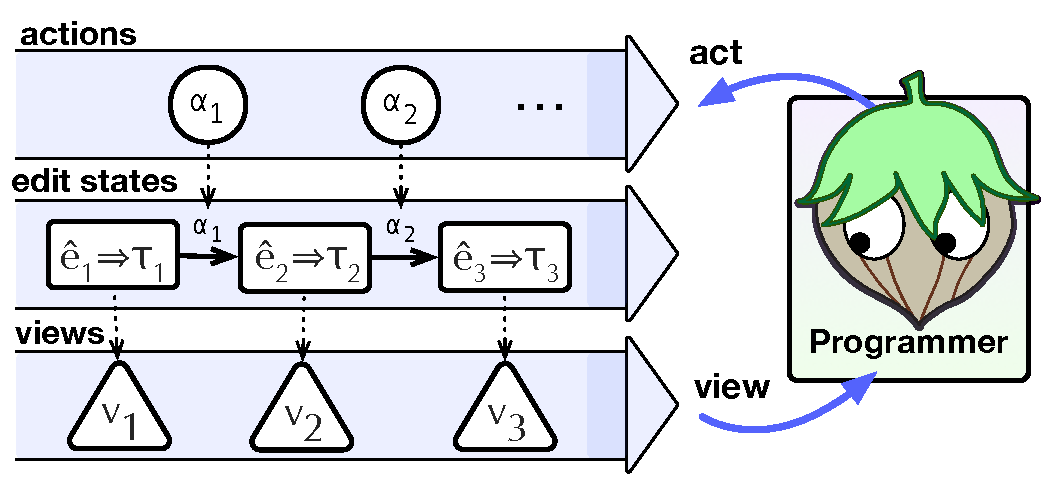
\includegraphics[width=0.90\columnwidth]{impl-overview2}
\caption{...}
\label{fig:impl-overview}
\end{figure}


\section{Related Work and Discussion}\label{sec:rw}
\subsection{Structure Editors}
Syntactic structure editors have a long history -- the Cornell Program
Synthesizer~\cite{teitelbaum_cornell_1981} was first introduced in
1981. Novice programmers have been a common target for structure
editors. For example, GNOME~\cite{garlan_gnome:_1984} was developed to
teach programming to undergraduates.
Alice~\cite{Conway:2000:ALL:332040.332481} is a 3-D programming language
with an integrated structure editor for teaching novice CS undergraduate
students. Scratch~\cite{Resnick:2009:SP:1592761.1592779} is a structure
editor targeted at children ages 8 to 16.
TouchDevelop \cite{tillmann_touchdevelop:_2011} incorporates a structure
editor for programming on touch-based devices, and is used to teach high
school students. An implementation of Hazelnut might be useful in teaching
students about the typed lambda calculus, though that has not been our
explicit aim with this work.

Not all structure editors are for educational purposes. For example,
mbeddr \cite{voelter_mbeddr:_2012} is a structure editor for a C-based
programming language (nominally, for programming embedded systems.)
Lamdu~\cite{lamdu}, like Hazelnut, is a structure editor for a statically
typed functional language. It is designed for use by professional
programmers.

The examples given so far either do not attempt to reason statically about
types and binding, or do not attempt to maintain well-typedness as an edit
invariant. This can pose problems, for reasons discussed in Sec. \ref{sec:introduction}. One apparent exception is Unison~\cite{unison}, a structure
editor for a typed functional language similar to Haskell. Like Hazelnut,
it seems to define some notion of well-typedness for expressions with holes
(though there is no technical documentation on virtually any aspect of its
design.) Unlike Hazelnut, it does not have a notion analogous to Hazelnut's
notion of a non-empty hole. As such, programmers must construct programs in
a rigid outside-in manner, as discussed in Sec. \ref{sec:example}. Another
system with the same problem is Polymorphic Blocks, a block-based user
interface where the structure of block connectors encodes a
type \cite{DBLP:conf/chi/LernerFG15}.

We fundamentally differ from these projects in our design philosophy: we
consider it essential to start by building type theoretic foundations,
which are independent of nearly all decisions about the user interface (other than our choice to use an explicit cursor.) In
contrast, these editors have developed innovative user interfaces (e.g. see
the discussion in \cite{DBLP:conf/sle/VolterSBK14}) but lack a principled
foundational calculus. In this respect, we follow the philosophical
approach taken by languages that are rooted in the type theoretic tradition
and have gone to great effort to develop a clear metatheory, like Standard
ML \cite{mthm97-for-dart,Harper00atype-theoretic,Lee:2007:TMM:1190216.1190245}.  In the future, we hope
that these lines of research will merge to produce a human-usable typed
structure editor with sound formal foundations. Our contribution, then, is
in defining and analyzing the theoretical properties of a small
foundational calculus that could be extended to achieve this vision.
Our implementation resembles the minimal structure editor defined in
Haskell by Sufrin and De Moor \cite{sufrin1999modeless}.


Some structure editor \emph{generators} do operate on formal or semi-formal
definitions of an underlying language. For example, the Synthesizer
Generator~\cite{Reps:1984:SG:390010.808247} allows the user to define an
attribute grammar-based language implementation that then can be used to
generate a structured editor. CENTAUR~\cite{Borras:1988:CS:64140.65005}
produces a language specific environment from a user defined formal
specification of a language. Barista is a programmatic toolkit for building
structure editors \cite{ko_barista:_2006}. mbeddr is built on top of the
commercial JetBrains MPS framework for constructing structure
editors \cite{voelter2011language,DBLP:journals/software/VoelterWK15}. These
systems do not give a semantics to the edit states of the structure editor
itself, or maintain non-trivial edit invariants, as Hazelnut does.

Related to structure editors are value editors, which operate directly on
simple values (but not generally expressions or functions) of a programming
language. For example, Eros is a typed value editor based in
Haskell \cite{DBLP:conf/icfp/Elliott07}.

Other work has attempted to integrate structure editing features into
text editors. For example, recent work has used syntactic placeholders
reminiscent of our expression holes to decrease the percentage of
edit states that are malformed \cite{Amorim:2016:PSC:2997364.2997374}. This work does not consider the semantics of placeholders.

Prior work has also explored
formal definitions of text editor commands, e.g. using functional
combinators \cite{DBLP:journals/scp/Sufrin82}.

\subsection{Gradual Type Systems}
A significant contribution of this paper is the discovery of a clear
technical relationship between typed structure editing and gradual
typing. In particular, the machinery necessary to give a reasonable
semantics to type holes -- i.e. type consistency and type matching --
coincides with that developed in the study of gradual type systems for
functional languages. The pioneering work of Siek and Taha \cite{Siek06a}
introduced type consistency. Subsequent work developed the concept of type
matching \cite{DBLP:conf/popl/RastogiCH12,DBLP:conf/popl/GarciaC15} and has further
studied the notion of type consistency \cite{Garcia:2016:AGT:2837614.2837670}. In
retrospect, this relationship is perhaps unsurprising: gradual typing is,
notionally, also motivated by the idea of iterated development of a program
where every intermediate state is well-defined in some sense, albeit at
different granularity.

Recent work has discovered a systematic procedure for generating a
``gradual version'' of a standard type
system \cite{DBLP:conf/popl/CiminiS16}. This system, called the
Gradualizer, operates on a logic program that specifies a simple type
assignment system with some additional annotations to generate a
corresponding specification of a gradual type system. The authors leave
support for working with bidirectional type systems as future work. This
suggests the possibility of an analogous ``Editorializer'' that generates a
specification of a typed structure editor from a simple language
definition. Our exposition in Sec. \ref{sec:extending} certainly suggests
that many of the necessary definitions follow seemingly mechanically from
the definition of the static semantics, and the relationship with gradual
typing suggests that many of the technical details of this transformation
may already exist in the Gradualizer. One possibility we have explored
informally is to use Agda's reflection features to implement such a system.

An aspect of gradual typing that we did not touch on directly here is its
concern with assigning a dynamics to programs where type information is not
known, by inserting dynamic type casts \cite{Siek06a} or deducing evidence for consistency during evaluation \cite{Garcia:2016:AGT:2837614.2837670}. This would correspond to assigning
a dynamics to Hazelnut expressions with type holes such that a run-time
error occurs when a type hole is found to be unfillable through evaluation. This
may be useful as an exploratory programming tool.

\subsection{Bidirectional Type Systems}
Hazelnut is bidirectionally typed \cite{Pierce:2000:LTI:345099.345100,DBLP:conf/icfp/DaviesP00,DBLP:conf/tldi/ChlipalaPH05,bidi-tutorial,odersky2001colored}. Bidirectional type systems are notable in
that they are easy to define, easy to implement, produce simple error messages and support advanced language features \cite{dunfield2013complete}. For example, Scala \cite{odersky2001colored} and Agda \cite{norell:thesis} are both fundamentally bidirectionally typed languages.


\subsection{Type Reconstruction}
An alternative approach to type inference is to use a unification-based type reconstruction system, as in functional languages like ML and Haskell \cite{damas1982principal}. This is difficult to reconcile with the approach presented in this paper, because edit actions could introduce new  unification constraints that would require placing non-empty holes around terms far from the cursor.  A whole-program hole insertion pass after each edit action could perhaps be used to recover invariants similar to those presented here, but we leave the details as future work. Our contention is that a bidirectional approach is a sweet spot in the design space of interactive systems like Hazelnut because it precludes
``spooky errors at a distance''. Instead, the interaction is a sort of local
dialog between the programmer and the system involving simple, familiar
concepts -- types with holes -- rather than sets of constraints.


An intermediate approach would be to
layer unification-based type generation features atop the bidirectional system. This would amount to  interpreting type holes as unification
variables. For a simple calculus,
e.g. the STLC upon which Hazelnut is based, type inference for complete expressions is known to be
decidable, so type holes could be instantiated automatically once the expression that they appear within has been constructed. It would also be possible to flag expressions for which there does not exist any way to fill the type holes. In more complex settings, e.g. in a
dependently typed language, a partial decision procedure may still be
useful in this regard, both at edit-time and (just prior to)
run-time. Indeed, text editor modes for dependently typed proof assistants, e.g. for Agda,
attempt to do exactly this for indicated ``type holes'' (and do not always
succeed.)

\subsection{Exceptions}
Expression holes can be interpreted in several
ways. One straightforward interpretation is to treat them
like expressions that raise exceptions. Indeed,
placing \textt{raise Unimplemented} or similar in portions of an expression
that are under construction is a common practice across programming
languages today. The GHC dialect of Haskell recently introduced an explicit notion of a
typed hole that behaves similarly \cite{GHC/holes}.

\subsection{Type-Directed Program Synthesis}
Some text editor modes, e.g. those for proof assistants like
Agda \cite{norell:thesis} and Idris \cite{brady2013idris}, support a more
explicit hole-based programming model where indicated expression holes are
treated as sites where the system can be asked to automatically generate an
expression of an appropriate type. %These systems are not statically
% well-defined themselves (though see below.)

The Graphite system borrowed Eclipse's heuristic model of typed holes for Java to allow
library providers to associate interactive code generation interfaces with
types \cite{Omar:2012:ACC:2337223.2337324}.

More generally, the topic of type-directed program synthesis an active area
of research, e.g. \cite{DBLP:conf/pldi/OseraZ15}. By maintaining static
well-definedness throughout the editing process, Hazelnut provides
researchers interested in editor-integrated type-directed program synthesis
with a formal foundation upon which to build.

\subsection{Tactics}

Interactive proof refinement systems, e.g. those in LCF \cite{Gordon:1978:MIP:512760.512773}, and more recent typed tactic systems, e.g. Mtac for Coq \cite{ziliani2015mtac},
support an explicit model of a ``current'' typed hole that serves as the
target of program synthesis. Hazelnut differs in that edits can occur anywhere within a term.


A related approach is to interpret expression holes as the \emph{metavariables} of contextual modal type theory
(CMTT) \cite{DBLP:journals/tocl/NanevskiPP08}. In particular, expression
holes have types and are surrounded by contexts, just as metavariables in
CMTT are associated with types and contexts. This begins to clarify the
logical meaning of a typing derivation in Hazelnut -- it conveys
well-typedness relative to an (implicit) modal context that extracts each
expression hole's type and context. The modal context must be emptied --
i.e. the expression holes must be instantiated with expressions of the
proper type in the proper context -- before the expression can be
considered complete. This corresponds to the notion of modal necessity in
contextual modal logic.

We did not make the modal context explicit in our semantics because interactive program editing is not
merely hole filling in Hazelnut (i.e. the cursor need not be on a
hole.) Moreover, the hole's type and context become apparent as our action
semantics traverses the zipper structure on each step. For interactive
proof assistants that support a tactic model based directly on hole
filling, as just discussed, the connection to CMTT and similar systems is more useful. For
example, Beluga \cite{DBLP:conf/flops/Pientka10} is based on dependent CMTT
and aspects of Idris' editor support \cite{brady2013idris} are based on
McBride's OLEG \cite{mcbride2000dependently} and Lee and Friedman have
explored a lambda calculus with contexts for a similar
purpose \cite{DBLP:conf/icfp/LeeF96}.

One interesting avenue of future work is to elaborate expression holes to
CMTT's closures, i.e. CMTT terms of the form
$\mathsf{clo}(u; \text{id}(\Gamma))$ where $u$ is a unique metavariable
associated with each hole and $\text{id}(\Gamma)$ is the explicit identity
substitution. This would allow us to evaluate expressions with holes such
that the closure ``accumulates'' substitutions explicitly. When evaluation
gets ``stuck'' (as it can, for CMTT does not define a dynamics equipped
with a notion of progress under a non-empty modal context), it would then
be possible for the programmer to choose a hole from the visible
holes (which may have been duplicated) to edit in their original
context. Once finished, the CMTT hole instantiation operation, together
with a metatheorem that establishes that reduction commutes with
instantiation, would enable an ``edit and resume'' feature with a clear
formal basis. This notion of reduction commuting with instantiation has
also been studied in other
calculi \cite{DBLP:journals/entcs/Sands97}. Being able to edit a running
program also has connections to less formal work on ``live programming''
interfaces \cite{burckhardt2013s,lamdu}.

\section{Conclusion}
\label{sec:future}
This paper presented Hazelnut, a type theoretic structure editor
calculus. Our aim was to take a principled approach to its design by
formally defining its static semantics as well as its action semantics and
developing a rich metatheory. Moreover, we have mechanized substantial
portions of the metatheory, including the crucial Sensibility theorem that
establishes that every edit state is statically meaningful.

In addition to simplifying the job of an editor designer, typed structure
editors also promise to increase the speed of development by eliminating
redundant syntax and supporting higher-level primitive actions. However, we
did not discuss such ``edit costs'' here, because they depend on particular
implementation details, e.g. whether a keyboard or a mouse is in
use. Indeed, we consider it a virtue of this work that such implementation
details do not enter into our design.

\subsection{Future Work}
\subsubsection{Richer Languages}
Hazelnut is, obviously, a very limited language at its core. So the most
obvious avenue for future work is to increase the expressive power of this
language by extension. Our plan is to simultaneously maintain a
mechanization and implementation (following, for example, Standard ML \cite{Lee:2007:TMM:1190216.1190245}) as
we proceed, ultimately producing the first large-scale, formally verified
bidirectionally typed structure editor.

It is interesting to note that the demarcation between the language and the
editor is fuzzy (indeed, non-existent) in Hazelnut. There may well be
interesting opportunities in language design when the language is being
codesigned with a typed structure editor. It may be that certain language
features are unnecessary given a sufficiently advanced type-aware structure
editor (e.g. SML's \texttt{open}?), while other features may only be
practical with editor support. We intend to use Hazelnut and derivative
systems thereof as a platform for rigorously exploring such questions.

\subsubsection{Evaluation Strategies: A High-Dimensional Space}
The related work brought up in the previous section suggests three different evaluation strategies in
the presence of type holes:
\begin{enumerate}[noitemsep]
\item ...as preventing evaluation (the standard approach.)
\item ...as unknown types, in the gradual sense.
\item ...as unification variables.
\end{enumerate}
In addition, we have discussed four different evaluation strategies in the
presence of expression holes:
\begin{enumerate}[noitemsep]
\item ...as preventing evaluation (the standard approach.)
\item ...as causing exceptions.
\item ...as sites for automatic program synthesis.
\item ...as the closures of CMTT.
\end{enumerate}

Every combination of these choices could well be considered in the design
of a full-scale programming system in the spirit of Hazelnut. Indeed, the
user might be given several options from among these combinations,
depending on their usage scenario. Many of these warrant further inquiry.


\subsubsection{Editor Services}
There are various aspects of the editor model that we have not yet
formalized. For example, our action model does not consider how actions are
actually entered using, for example, key combinations or chords. In
practice, we would want also to suggest sensible compound actions, and
to rank these suggested actions in some reasonable
manner (perhaps based on usage data gathered from other users or code
repositories.) Designing a action suggestion semantics and a rigorous typed probability model over actions is one avenue of research that we have started to
explore, with intriguing initial results.

\subsubsection{Programmable Actions}
Our language of actions is intentionally primitive. However, even now it
acts much like a simple imperative command language. This suggests future
expansion to, for example, a true \emph{action macro} language, whereby
functional programs could themselves be lifted to the level of actions to
compute non-trivial compound actions. Such compound actions would give a
uniform description of transformations ranging from the simple -- like
``move the cursor to the next hole to the right'' -- to quite complex whole
program refactoring, while remaining subject to the core Hazelnut
metatheory. Techniques like those in advanced tactic systems, e.g. Mtac, might be useful
in proving these action macros correct \cite{ziliani2015mtac}.

\subsubsection{Views}
Another research direction is in exploring how types can be used to control
the presentation of expressions in the editor. For example, following an
approach developed in a textual setting of developing \emph{type-specific
languages} (TSLs), it should be possible to have the type that an
expression is being analyzed against define alternative display forms and
interaction modes \cite{TSLs}.

It should also be possible to develop the concept of semantic comments,
i.e. comments that mention semantic structures or even contain values. These would be subject to
the same operations, e.g. renaming, as other structures, helping to address
the problem of comments becoming inconsistent with code. This system, generalized sufficiently,
could one day help unify document editing with program editing.

\subsubsection{Collaborative Programming}
Finally, we did not consider any aspects of \emph{collaborative
programming}, such as a packaging system, a differencing algorithm for use
in a source control system, support for multiple simultaneous cursors for
different users, and so on. These are all interesting avenues for future
work.

\subsubsection{Empirical Evaluation}
Although we make few empirical claims in this paper, it is ultimately an
empirical question as to whether structure editors, and typed structure
editors, are practical. We hope to conduct user studies once a richer
semantics and a practical implementation thereof has been developed.

\subsubsection{More Theory}
Connections with gradual type systems and CMTT, discussed in the previous
section, seem likely to continue to be revealing.

The notion of having one of many possible locations within a term under a
cursor has a very strong intuitive connection to the proof theoretic notion
of focusing \cite{Simmons11tr}. Building closer connections with proof
theory (and category theory) is likely to be a fruitful avenue of further
inquiry.

\begin{quote}
\emph{In any case, these are but steps toward more graphical program-description
systems, for we will not forever stay confined to mere strings of symbols.}

--- Marvin Minsky, Turing Award lecture \cite{DBLP:journals/jacm/Minsky70}
\end{quote}

\acks
% !TEX root = hazelnut-popl17.tex

The authors would like to thank the anonymous referees at POPL and TFP 2016  for useful feedback on earlier drafts of this paper; Ed Morehouse and Carlo Angiuli for counsel on mechanization and Barendrecht's
Convention; Vincent Zeng for \textit{pro bono} artistic services; and YoungSeok Yoon for reanalyzing the data from \cite{6883030}. 
%This is Danny Dig's COPE grant. He asked me to add the grant.
This work was partially funded through the NSF grant \#CCF-1439957; by AFRL and DARPA under agreement \#FA8750-16-2-0042; and by NSA lablet contract \#H98230-14-C-0140. The views and conclusions contained herein are those of the authors and should not be interpreted as necessarily representing the official policies or endorsements, either expressed or implied, of the NSF, AFRL, DARPA, the NSA or the U.S. Government.


\balance
\bibliographystyle{abbrvnat}
% The bibliography should be embedded for final submission.
\bibliography{bibliography}

\iftr
\clearpage
\onecolumn
\appendix
% !TEX root = hazelnut-popl17.tex

\section{Hazelnut}
The full collection of rules defining the semantics of Hazelnut are
reproduced here in their definitional order for reference, omitting only
the rules for binary sums. The names given coincide with the corresponding
constructors in the Agda formalization.
\subsection{H-Types and H-Expressions}
\subsubsection{Type Compatibility and Incompatibility}

\noindent\fbox{$\tcompat{\htau}{\htau'}$}
\begin{subequations}
  \begin{equation}
    \tag{\rname{TCRefl}}
    \inferrule{ }{
      \tcompat{\htau}{\htau}
    }
  \end{equation}
  \gap{}
  \begin{equation}
    \tag{\rname{TCHole1}}
    \inferrule{ }{
      \tcompat{\htau}{\tehole}
    }
  \end{equation}
  \gap{}
  \begin{equation}
    \tag{\rname{TCHole2}}
    \inferrule{ }{
      \tcompat{\tehole}{\htau}
    }
  \end{equation}
  \gap{}
  \begin{equation}
    \tag{\rname{TCArr}}
    \inferrule{
      \tcompat{\htau_1}{\htau_1'}\\
      \tcompat{\htau_2}{\htau_2'}
    }{
      \tcompat{\tarr{\htau_1}{\htau_2}}{\tarr{\htau_1'}{\htau_2'}}
    }
  \end{equation}
\end{subequations}

\noindent\fbox{$\tincompat{\htau}{\htau'}$}
\begin{subequations}
  \begin{equation}
    \tag{\rname{ICNumArr1}}
    \inferrule{ }{
      \tincompat{\tnum}{\tarr{\htau_1}{\htau_2}}
    }
  \end{equation}
  \gap{}
  \begin{equation}
    \tag{\rname{ICNumArr2}}
    \inferrule{ }{
      \tincompat{\tarr{\htau_1}{\htau_2}}{\tnum}
    }
  \end{equation}
  \gap{}
  \begin{equation}
    \tag{\rname{ICArr1}}
    \inferrule{
      \tincompat{\htau_1}{\htau_3}
    }{
      \tincompat{\tarr{\htau_1}{\htau_2}}{\tarr{\htau_3}{\htau_4}}
    }
  \end{equation}
  \gap{}
  \begin{equation}
    \tag{\rname{ICArr2}}
    \inferrule{
      \tincompat{\htau_2}{\htau_4}
    }{
      \tincompat{\tarr{\htau_1}{\htau_2}}{\tarr{\htau_3}{\htau_4}}
    }
  \end{equation}
\end{subequations}

\subsubsection{Function Type Matching}~
\noindent
\fbox{$\arrmatch{\htau}{\tarr{\htau_1}{\htau_2}}$}~~\text{$\tau$ has
  matched arrow type $\tarr{\htau_1}{\htau_2}$}
\begin{subequations}
  \begin{equation}
    \tag{\rname{MAHole}}
    \inferrule{ }{
      \arrmatch{\tehole}{\tarr{\tehole}{\tehole}}
    }
  \end{equation}
  \gap{}
  \begin{equation}
    \tag{\rname{MAArr}}
    \inferrule{ }{
      \arrmatch{\tarr{\htau_1}{\htau_2}}{\tarr{\htau_1}{\htau_2}}
    }
  \end{equation}
\end{subequations}

\subsubsection{Synthesis and Analysis}
The judgements $\hsyn{\hGamma}{\hexp}{\htau}$ and
$\hana{\hGamma}{\hexp}{\htau}$ are defined mutually inductively by Rules
(\ref{Arules:hsyn}) and Rules (\ref{Arules:hana}), respectively.

\noindent\fbox{$\hsyn{\hGamma}{\hexp}{\htau}$}~~\text{$\hexp$ synthesizes $\htau$}
\begin{subequations}\label{Arules:hsyn}
  \begin{equation}
    \tag{\rname{SAsc}}
    \inferrule{
      \hana{\hGamma}{\hexp}{\htau}
    }{
      \hsyn{\hGamma}{\hexp : \htau}{\htau}
    }
  \end{equation}
  \gap{}
  \begin{equation}
    \tag{\rname{SVar}}
    \inferrule{ }{
      \hsyn{\hGamma, x : \htau}{x}{\htau}
    }
  \end{equation}
  \gap{}
  \begin{equation}
    \tag{\rname{SAp}}
    \inferrule{
      \hsyn{\hGamma}{\hexp_1}{\htau}\\
      \arrmatch{\htau}{\tarr{\htau_2}{\htau'}}\\
      \hana{\hGamma}{\hexp_2}{\htau_2}
    }{
      \hsyn{\hGamma}{\hap{\hexp_1}{\hexp_2}}{\htau'}
    }
  \end{equation}
  \gap{}
  \begin{equation}
    \tag{\rname{SNum}}
    \inferrule{ }{
      \hsyn{\hGamma}{\hnum{n}}{\tnum}
    }
  \end{equation}
  \gap{}
  \begin{equation}
    \tag{\rname{SPlus}}
    \inferrule{
      \hana{\hGamma}{\hexp_1}{\tnum}\\
      \hana{\hGamma}{\hexp_2}{\tnum}
    }{
      \hsyn{\hGamma}{\hadd{\hexp_1}{\hexp_2}}{\tnum}
    }
  \end{equation}
  \gap{}
  \begin{equation}
    \tag{\rname{SHole}}
    \inferrule{ }{
      \hsyn{\hGamma}{\hehole}{\tehole}
    }
  \end{equation}
  \gap{}
  \begin{equation}
    \tag{\rname{SNEHole}}
    \inferrule{
      \hsyn{\hGamma}{\hexp}{\htau}
    }{
      \hsyn{\hGamma}{\hhole{\hexp}}{\tehole}
    }
  \end{equation}
\end{subequations}
\noindent\fbox{$\hana{\hGamma}{\hexp}{\htau}$}~~\text{$\hexp$ analyzes against $\htau$}
\begin{subequations}\label{Arules:hana}
  \begin{equation}
    \tag{\rname{ASubsume}}
    \inferrule{
      \hsyn{\hGamma}{\hexp}{\htau'}\\
      \tcompat{\htau}{\htau'}
    }{
      \hana{\hGamma}{\hexp}{\htau}
    }
  \end{equation}
  \gap{}
  \begin{equation}
    \tag{\rname{ALam}}
    \inferrule{
      \arrmatch{\htau}{\tarr{\htau_1}{\htau_2}}\\
      \hana{\hGamma, x : \htau_1}{\hexp}{\htau_2}
    }{
      \hana{\hGamma}{\hlam{x}{\hexp}}{\htau}
    }
  \end{equation}
\end{subequations}

\subsection{Z-Types and Z-Expressions}
\subsubsection{Type Focus Erasure}
\noindent\fbox{$\removeSel{\ztau}=\htau$} is a metafunction defined as follows:
\begin{subequations}
  \begin{align}
    \tag{\rname{ETTop}}
    \removeSel{\zwsel{\htau}} & = \htau\\
    \tag{\rname{ETArrL}}
    \removeSel{\tarr{\ztau}{\htau}} & = \tarr{\removeSel{\ztau}}{\htau}\\
    \tag{\rname{ETArrR}}
    \removeSel{\tarr{\htau}{\ztau}} & = \tarr{\htau}{\removeSel{\ztau}}
  \end{align}
\end{subequations}

\subsubsection{Expression Focus Erasure}
\noindent\fbox{$\removeSel{\zexp}=\hexp$} is a metafunction defined as follows:
\begin{subequations}
  \begin{align}
    \tag{\rname{EETop}}
    \removeSel{\zwsel{\hexp}} & = \hexp\\
    \tag{\rname{EEAscL}}
    \removeSel{\zexp : \htau} & = \removeSel{\zexp} : \htau\\
    \tag{\rname{EEAscR}}
    \removeSel{\hexp : \ztau} & = \hexp : \removeSel{\ztau}\\
    \tag{\rname{EELam}}
    \removeSel{\hlam{x}{\zexp}} & = \hlam{x}{\removeSel{\zexp}}\\
    \tag{\rname{EEApL}}
    \removeSel{\hap{\zexp}{\hexp}} & = \hap{\removeSel{\zexp}}{\hexp}\\
    \tag{\rname{EEApR}}
    \removeSel{\hap{\hexp}{\zexp}} & = \hap{\hexp}{\removeSel{\zexp}}\\
    \tag{\rname{EEPlusL}}
    \removeSel{\hadd{\zexp}{\hexp}} & = \hadd{\removeSel{\zexp}}{\hexp}\\
    \tag{\rname{EEPlusR}}
    \removeSel{\hadd{\hexp}{\zexp}} & = \hadd{\hexp}{\removeSel{\zexp}}\\
    \tag{\rname{EENEHole}}
    \removeSel{\hhole{\zexp}} &= \hhole{\removeSel{\zexp}}
  \end{align}
\end{subequations}

\subsection{Action Model}
\subsubsection{Type Actions}
\noindent\fbox{$\performTyp{\ztau}{\alpha}{\ztau'}$}
\paragraph{Type Movement}
\begin{subequations}
  \begin{equation}
    \tag{\rname{TMArrChild1}}
    \inferrule{ }{
      \performTyp{
        \zwsel{\tarr{\htau_1}{\htau_2}}
      }{
        \aMove{\dChildn{1}}
      }{
        \tarr{\zwsel{\htau_1}}{\htau_2}
      }
    }
  \end{equation}
  \gap{}
  \begin{equation}
    \tag{\rname{TMArrChild2}}
    \inferrule{ }{
      \performTyp{
        \zwsel{\tarr{\htau_1}{\htau_2}}
      }{
        \aMove{\dChildn{2}}
      }{
        \tarr{\htau_1}{\zwsel{\htau_2}}
      }
    }
  \end{equation}
  \gap{}
  \begin{equation}
    \tag{\rname{TMArrParent1}}
    \inferrule{ }{
      \performTyp{
        \tarr{\zwsel{\htau_1}}{\htau_2}
      }{
        \aMove{\dParent}
      }{
        \zwsel{\tarr{\htau_1}{\htau_2}}
      }
    }
  \end{equation}
  \gap{}
  \begin{equation}
    \tag{\rname{TMArrParent2}}
    \inferrule{ }{
      \performTyp{
        \tarr{{\htau_1}}{\zwsel{\htau_2}}
      }{
        \aMove{\dParent}
      }{
        \zwsel{\tarr{\htau_1}{\htau_2}}
      }
    }
  \end{equation}

  \paragraph{Type Deletion}
  \begin{equation}
    \tag{\rname{TMDel}}
    \inferrule{ }{
      \performTyp{
        \zwsel{\htau}
      }{
        \aDel
      }{
        \zwsel{\tehole}
      }
    }
  \end{equation}

  \paragraph{Type Construction}
  \begin{equation}
    \tag{\rname{TMConArrow}}
    \inferrule{ }{
      \performTyp{
        \zwsel{\htau}
      }{
        \aConstruct{\farr}
      }{
        \tarr{\htau}{\zwsel{\tehole}}
      }
    }
  \end{equation}
  \gap{}
  \begin{equation}
    \tag{\rname{TMConNum}}
    \inferrule{ }{
      \performTyp{
        \zwsel{\tehole}
      }{
        \aConstruct{\fnum}
      }{
        \zwsel{\tnum}
      }
    }
  \end{equation}

  \paragraph{Zipper Cases}
  \begin{equation}
    \tag{\rname{TMArrZip1}}
    \inferrule{
      \performTyp{\ztau}{\alpha}{\ztau'}
    }{
      \performTyp{
        \tarr{\ztau}{\htau}
      }{
        \alpha
      }{
        \tarr{\ztau'}{\htau}
      }
    }
  \end{equation}
  \gap{}
  \begin{equation}
    \tag{\rname{TMArrZip2}}
    \inferrule{
      \performTyp{\ztau}{\alpha}{\ztau'}
    }{
      \performTyp{
        \tarr{\htau}{\ztau}
      }{
        \alpha
      }{
        \tarr{\htau}{\ztau'}
      }
    }
  \end{equation}
\end{subequations}

\subsubsection{Expression Movement Actions}
\noindent\fbox{$\performMove{\zexp}{\aMove{\delta}}{\zexp'}$}

\begin{subequations}
  \paragraph{Ascription}
  \begin{equation}
    \tag{\rname{EMAscChild1}}
    \inferrule{ }{
      \performTyp{
        \zwsel{\hexp : \htau}
      }{
        \aMove{\dChildn{1}}
      }{
        \zwsel{\hexp} : \htau
      }
    }
  \end{equation}
  \gap{}
  \begin{equation}
    \tag{\rname{EMAscChild2}}
    \inferrule{ }{
      \performTyp{
        \zwsel{\hexp : \htau}
      }{
        \aMove{\dChildn{2}}
      }{
        \hexp : \zwsel{\htau}
      }
    }
  \end{equation}
  \gap{}
  \begin{equation}
    \tag{\rname{EMAscParent1}}
    \inferrule{ }{
      \performTyp{
        \zwsel{\hexp} : \htau
      }{
        \aMove{\dParent}
      }{
        \zwsel{\hexp : \htau}
      }
    }
  \end{equation}
  \gap{}
  \begin{equation}
    \tag{\rname{EMAscParent2}}
    \inferrule{ }{
      \performTyp{
        \hexp : \zwsel{\htau}
      }{
        \aMove{\dParent}
      }{
        \zwsel{\hexp : \htau}
      }
    }
  \end{equation}

  \paragraph{Lambda}
  \begin{equation}
    \tag{\rname{EMLamChild1}}
    \inferrule{ }{
      \performMove{
        \zwsel{\hlam{x}{\hexp}}
      }{
        \aMove{\dChildn{1}}
      }{
        \hlam{x}{\zwsel{\hexp}}
      }
    }
  \end{equation}
  \gap{}
  \begin{equation}
    \tag{\rname{EMLamParent}}
    \inferrule{ }{
      \performMove{
        \hlam{x}{\zwsel{\hexp}}
      }{
        \aMove{\dParent}
      }{
        \zwsel{\hlam{x}{\hexp}}
      }
    }
  \end{equation}

  \paragraph{Plus}
  \begin{equation}
    \tag{\rname{EMPlusChild1}}
    \inferrule{ }{
      \performMove{
        \zwsel{\hadd{\hexp_1}{\hexp_2}}
      }{
        \aMove{\dChildn{1}}
      }{
        \hadd{\zwsel{\hexp_1}}{\hexp_2}
      }
    }
  \end{equation}
  \gap{}
  \begin{equation}
    \tag{\rname{EMPlusChild2}}
    \inferrule{ }{
      \performMove{
        \zwsel{\hadd{\hexp_1}{\hexp_2}}
      }{
        \aMove{\dChildn{2}}
      }{
        \hadd{\hexp_1}{\zwsel{\hexp_2}}
      }
    }
  \end{equation}
  \gap{}
  \begin{equation}
    \tag{\rname{EMPlusParent1}}
    \inferrule{ }{
      \performMove{
        \hadd{\zwsel{\hexp_1}}{\hexp_2}
      }{
        \aMove{\dParent}
      }{
        \zwsel{\hadd{\hexp_1}{\hexp_2}}
      }
    }
  \end{equation}
  \gap{}
  \begin{equation}
    \tag{\rname{EMPlusParent2}}
    \inferrule{ }{
      \performMove{
        \hadd{{\hexp_1}}{\zwsel{\hexp_2}}
      }{
        \aMove{\dParent}
      }{
        \zwsel{\hadd{\hexp_1}{\hexp_2}}
      }
    }
  \end{equation}

  \paragraph{Application}
  \begin{equation}
    \tag{\rname{EMApChild1}}
    \inferrule{ }{
      \performMove{
        \zwsel{\hap{\hexp_1}{\hexp_2}}
      }{
        \aMove{\dChildn{1}}
      }{
        \hap{\zwsel{\hexp_1}}{\hexp_2}
      }
    }
  \end{equation}
  \gap{}
  \begin{equation}
    \tag{\rname{EMApChild2}}
    \inferrule{ }{
      \performMove{
        \zwsel{\hap{\hexp_1}{\hexp_2}}
      }{
        \aMove{\dChildn{2}}
      }{
        \hap{\hexp_1}{\zwsel{\hexp_2}}
      }
    }
  \end{equation}
  \gap{}
  \begin{equation}
    \tag{\rname{EMApParent1}}
    \inferrule{ }{
      \performMove{
        \hap{\zwsel{\hexp_1}}{\hexp_2}
      }{
        \aMove{\dParent}
      }{
        \zwsel{\hap{\hexp_1}{\hexp_2}}
      }
    }
  \end{equation}
  \gap{}
  \begin{equation}
    \tag{\rname{EMApParent2}}
    \inferrule{ }{
      \performMove{
        \hap{{\hexp_1}}{\zwsel{\hexp_2}}
      }{
        \aMove{\dParent}
      }{
        \zwsel{\hap{\hexp_1}{\hexp_2}}
      }
    }
  \end{equation}

  \paragraph{Non-Empty Hole}
  \begin{equation}
    \tag{\rname{EMNEHoleChild1}}
    \inferrule{ }{
      \performMove{
        \zwsel{\hhole{\hexp}}
      }{
        \aMove{\dChildn{1}}
      }{
        \hhole{\zwsel{\hexp}}
      }
    }
  \end{equation}
  \begin{equation}
    \tag{\rname{EMNEHoleParent}}
    \inferrule{ }{
      \performMove{
        \hhole{\zwsel{\hexp}}
      }{
        \aMove{\dParent}
      }{
        \zwsel{\hhole{\hexp}}
      }
    }
  \end{equation}

\end{subequations}
\subsubsection{Synthetic and Analytic Expression Actions}
The synthetic and analytic expression action performance judgements are
defined mutually inductively by Rules (\ref{Arules:performSyn}) and Rules
(\ref{Arules:performAna}), respectively.

\noindent\fbox{$\performSyn{\hGamma}{\zexp}{\htau}{\alpha}{\zexp'}{\htau'}$}

\begin{subequations}\label{Arules:performSyn}
  \paragraph{Movement}
  \begin{equation}
    \tag{\rname{SAMove}}
    \inferrule{
      \performMove{\zexp}{\aMove{\delta}}{\zexp'}
    }{
      \performSyn{\hGamma}{\zexp}{\htau}{\aMove{\delta}}{\zexp'}{\htau}
    }
  \end{equation}

  \paragraph{Deletion}
  \begin{equation}
    \tag{\rname{SADel}}
    \inferrule{ }{
      \performSyn{\hGamma}{\zwsel{\hexp}}{\htau}{\aDel}{\zwsel{\hehole}}{\tehole}
    }
  \end{equation}

  \paragraph{Construction}
  \begin{equation}
    \tag{\rname{SAConAsc}}
    \inferrule{ }{
      \performSyn{\hGamma}{\zwsel{\hexp}}{\htau}{\aConstruct{\fasc}}{\hexp : \zwsel{\htau}}{\htau}
    }
  \end{equation}
  \gap{}
  \begin{equation}
    \tag{\rname{SAConVar}}
    \inferrule{ }{
      \performSyn{\hGamma, x : \htau}{\zwsel{\hehole}}{\tehole}{\aConstruct{\fvar{x}}}{\zwsel{x}}{\htau}
    }
  \end{equation}
  \gap{}
  \begin{equation}
    \tag{\rname{SAConLam}}
    \inferrule{ }{
      \performSyn
          {\hGamma}
          {\zwsel{\hehole}}
          {\tehole}
          {\aConstruct{\flam{x}}}
          {\hlam{x}{\hehole} : \tarr{\zwsel{\tehole}}{\tehole}}
          {\tarr{\tehole}{\tehole}}
    }
  \end{equation}
  \gap{}
  \begin{equation}
    \tag{\rname{SAConApArr}}
    \inferrule{
      \arrmatch{\htau}{\tarr{\htau_1}{\htau_2}}
    }{
      \performSyn
          {\hGamma}
          {\zwsel{\hexp}}
          {\htau}
          {\aConstruct{\fap}}
          {\hap{\hexp}{\zwsel{\hehole}}}
          {\htau_2}
    }
  \end{equation}
  \gap{}
  \begin{equation}
    \tag{\rname{SAConApOtw}}
    \inferrule{
      \tincompat{\htau}{\tarr{\tehole}{\tehole}}
    }{
      \performSyn
          {\hGamma}
          {\zwsel{\hexp}}
          {\htau}
          {\aConstruct{\fap}}
          {\hap{\hhole{\hexp}}{\zwsel{\hehole}}}
          {\tehole}
    }
  \end{equation}
  \gap{}
  \begin{equation}
    \tag{\rname{SAConNumLit}}
    \inferrule{ }{
      \performSyn
          {\hGamma}
          {\zwsel{\hehole}}
          {\tehole}
          {\aConstruct{\fnumlit{n}}}
          {\zwsel{\hnum{n}}}
          {\tnum}
    }
  \end{equation}
  \gap{}
  \begin{equation}
    \tag{\rname{SAConPlus1}}
    \inferrule{
      \tcompat{\htau}{\tnum}
    }{
      \performSyn
          {\hGamma}
          {\zwsel{\hexp}}
          {\htau}
          {\aConstruct{\fplus}}
          {\hadd{\hexp}{\zwsel{\hehole}}}
          {\tnum}
    }
  \end{equation}
  \gap{}
  \begin{equation}
    \tag{\rname{SAConPlus2}}
    \inferrule{
      \tincompat{\htau}{\tnum}
    }{
      \performSyn
          {\hGamma}
          {\zwsel{\hexp}}
          {\htau}
          {\aConstruct{\fplus}}
          {\hadd{\hhole{\hexp}}{\zwsel{\hehole}}}
          {\tnum}
    }
  \end{equation}
  \gap{}
  \begin{equation}
    \tag{\rname{SAConNEHole}}
    \inferrule{ }{
      \performSyn
          {\hGamma}
          {\zwsel{\hexp}}
          {\htau}
          {\aConstruct{\fnehole}}
          {\hhole{\zwsel{\hexp}}}
          {\tehole}
    }
  \end{equation}

  \paragraph{Finishing}
  \begin{equation}
    \tag{\rname{SAFinish}}
    \inferrule{
      \hsyn{\hGamma}{\hexp}{\htau'}
    }{
      \performSyn
          {\hGamma}
          {\zwsel{\hhole{\hexp}}}
          {\tehole}
          {\aFinish}
          {\zwsel{\hexp}}
          {\htau'}
    }
  \end{equation}

  \paragraph{Zipper Cases}
  \begin{equation}
    \tag{\rname{SAZipAsc1}}
    \inferrule{
      \performAna
          {\hGamma}
          {\zexp}
          {\htau}
          {\alpha}
          {\zexp'}
    }{
      \performSyn
          {\hGamma}
          {\zexp : \htau}
          {\htau}
          {\alpha}
          {\zexp' : \htau}
          {\htau}
    }
  \end{equation}
  \gap{}
  \begin{equation}
    \tag{\rname{SAZipAsc2}}
    \inferrule{
      \performTyp{\ztau}{\alpha}{\ztau'}\\
      \hana{\hGamma}{\hexp}{\removeSel{\ztau'}}
    }{
      \performSyn
          {\hGamma}
          {\hexp : \ztau}
          {\removeSel{\ztau}}
          {\alpha}
          {\hexp : \ztau'}
          {\removeSel{\ztau'}}
    }
  \end{equation}
  \gap{}
  \begin{equation}
    \tag{\rname{SAZipApArr}}
    \inferrule{
      \hsyn{\hGamma}{\removeSel{\zexp}}{\htau_2}\\
      \performSyn
          {\hGamma}
          {\zexp}
          {\htau_2}
          {\alpha}
          {\zexp'}
          {\htau_3}\\\\
          \arrmatch{\htau_3}{\tarr{\htau_4}{\htau_5}}\\
          \hana{\hGamma}{\hexp}{\htau_4}
    }{
      \performSyn
          {\hGamma}
          {\hap{\zexp}{\hexp}}
          {\htau_1}
          {\alpha}
          {\hap{\zexp'}{\hexp}}
          {\htau_5}
    }
  \end{equation}
  \gap{}
  \begin{equation}
    \tag{\rname{SAZipApAna}}
    \inferrule{
      \hsyn{\hGamma}{\hexp}{\htau_2}\\
      \arrmatch{\htau_2}{\tarr{\htau_3}{\htau_4}}\\
      \performAna
          {\hGamma}
          {\zexp}
          {\htau_3}
          {\alpha}
          {\zexp'}
    }{
      \performSyn
          {\hGamma}
          {\hap{\hexp}{\zexp}}
          {\htau_1}
          {\alpha}
          {\hap{\hexp}{\zexp'}}
          {\htau_4}
    }
  \end{equation}
  \gap{}
  \begin{equation}
    \tag{\rname{SAZipPlus1}}
    \inferrule{
      \performAna
          {\hGamma}
          {\zexp}
          {\tnum}
          {\alpha}
          {\zexp'}
    }{
      \performSyn
          {\hGamma}
          {\hadd{\zexp}{\hexp}}
          {\tnum}
          {\alpha}
          {\hadd{\zexp'}{\hexp}}
          {\tnum}
    }
  \end{equation}
  \gap{}
  \begin{equation}
    \tag{\rname{SAZipPlus2}}
    \inferrule{
      \performAna
          {\hGamma}
          {\zexp}
          {\tnum}
          {\alpha}
          {\zexp'}
    }{
      \performSyn
          {\hGamma}
          {\hadd{\hexp}{\zexp}}
          {\tnum}
          {\alpha}
          {\hadd{\hexp}{\zexp'}}
          {\tnum}
    }
  \end{equation}
  \gap{}
  \begin{equation}
    \tag{\rname{SAZipHole}}
    \inferrule{
      \hsyn{\hGamma}{\removeSel{\zexp}}{\htau}\\
      \performSyn
          {\hGamma}
          {\zexp}
          {\htau}
          {\alpha}
          {\zexp'}
          {\htau'}
    }{
      \performSyn
          {\hGamma}
          {\hhole{\zexp}}
          {\tehole}
          {\alpha}
          {\hhole{\zexp'}}
          {\tehole}
    }
  \end{equation}
\end{subequations}

\noindent\fbox{$\performAna{\hGamma}{\zexp}{\htau}{\alpha}{\zexp'}$}
\begin{subequations}\label{Arules:performAna}
  \paragraph{Subsumption}
  \begin{equation}
    \tag{\rname{AASubsume}}
    \inferrule{
      \hsyn{\hGamma}{\removeSel{\zexp}}{\htau'}\\
      \performSyn{\hGamma}{\zexp}{\htau'}{\alpha}{\zexp'}{\htau''}\\
      \tcompat{\htau}{\htau''}%\\\\
    }{
      \performAna{\hGamma}{\zexp}{\htau}{\alpha}{\zexp'}
    }
  \end{equation}

  \paragraph{Movement}
  \begin{equation}
    \tag{\rname{AAMove}}
    \inferrule{
      \performMove{\zexp}{\aMove{\delta}}{\zexp'}
    }{
      \performAna{\hGamma}{\zexp}{\htau}{\aMove{\delta}}{\zexp'}
    }
  \end{equation}

  \paragraph{Deletion}
  \begin{equation}
    \tag{\rname{AADel}}
    \inferrule{ }{
      \performAna{\hGamma}{\zwsel{\hexp}}{\htau}{\aDel}{\zwsel{\hehole}}
    }
  \end{equation}

  \paragraph{Construction}
  \begin{equation}
    \tag{\rname{AAConAsc}}
    \inferrule{ }{
      \performAna{\hGamma}{\zwsel{\hexp}}{\htau}{\aConstruct{\fasc}}{\hexp : \zwsel{\htau}}
    }
  \end{equation}
  \gap{}
  \begin{equation}
    \tag{\rname{AAConVar}}
    \inferrule{
      \tincompat{\htau}{\htau'}
    }{
      \performAna{\hGamma, x : \htau'}{\zwsel{\hehole}}{\htau}{\aConstruct{\fvar{x}}}{\hhole{\zwsel{x}}}
    }
  \end{equation}
  \gap{}
  \begin{equation}
    \tag{\rname{AAConLam1}}
    \inferrule{
      \arrmatch{\htau}{\tarr{\htau_1}{\htau_2}}
    }{
      \performAna
          {\hGamma}
          {\zwsel{\hehole}}
          {\htau}
          {\aConstruct{\flam{x}}}
          {\hlam{x}{\zwsel{\hehole}}}
    }
  \end{equation}
  \gap{}
  \begin{equation}
    \tag{\rname{AAConLam2}}
    \inferrule{
      \tincompat{\htau}{\tarr{\tehole}{\tehole}}
    }{
      \performAna
          {\hGamma}
          {\zwsel{\hehole}}
          {\htau}
          {\aConstruct{\flam{x}}}
          {\hhole{
              \hlam{x}{\hehole} : \tarr{\zwsel{\tehole}}{\tehole}
          }}
    }
  \end{equation}
  \gap{}
  \begin{equation}
    \tag{\rname{AAConNumLit}}
    \inferrule{
      \tincompat{\htau}{\tnum}
    }{
      \performAna
          {\hGamma}
          {\zwsel{\hehole}}
          {\htau}
          {\aConstruct{\fnumlit{n}}}
          {\hhole{\zwsel{\hnum{n}}}}
    }
  \end{equation}

  \paragraph{Finishing}
  \begin{equation}
    \tag{\rname{AAFinish}}
    \inferrule{
      \hana{\hGamma}{\hexp}{\htau}
    }{
      \performAna
          {\hGamma}
          {\zwsel{\hhole{\hexp}}}
          {\htau}
          {\aFinish}
          {\zwsel{\hexp}}
    }
  \end{equation}

  \paragraph{Zipper Cases}
  \begin{equation}
    \tag{\rname{AAZipLam}}
    \inferrule{
      \arrmatch{\htau}{\tarr{\htau_1}{\htau_2}}\\
      \performAna
          {\hGamma, x : \htau_1}
          {\zexp}
          {\htau_2}
          {\alpha}
          {\zexp'}
    }{
      \performAna
          {\hGamma}
          {\hlam{x}{\zexp}}
          {\htau}
          {\alpha}
          {\hlam{x}{\zexp'}}
    }
  \end{equation}
\end{subequations}
\subsubsection{Iterated Action Judgements} ~

\noindent $\mathsf{ActionList}$~~$\bar{\alpha} ::= \cdot ~\vert~ \alpha; \bar{\alpha}$\vspace{4px}\\
\fbox{$\performTypI{\ztau}{\bar{\alpha}}{\ztau'}$}
\begin{subequations}
  \begin{equation}
    \tag{\rname{DoRefl}}
    \inferrule{ }{
      \performTypI{\ztau}{\cdot}{\ztau}
    }
  \end{equation}
  \gap{}
  \begin{equation}
    \tag{\rname{DoType}}
    \inferrule{
      \performTyp{\ztau}{\alpha}{\ztau'}\\
      \performTypI{\ztau'}{\bar{\alpha}}{\ztau''}
    }{
      \performTypI{\ztau}{\alpha; \bar{\alpha}}{\ztau''}
    }
  \end{equation}
\end{subequations}

\begin{subequations}
  \fbox{$\performSynI{\hGamma}{\zexp}{\htau}{\bar{\alpha}}{\zexp'}{\htau'}$}
  \begin{equation}
    \tag{\rname{DoRefl}}
    \inferrule{ }{
      \performSynI{\hGamma}{\zexp}{\htau}{\cdot}{\zexp}{\htau}
    }
  \end{equation}
  \gap{}
  \begin{equation}
    \tag{\rname{DoSynth}}
    \inferrule{
      \performSyn{\hGamma}{\zexp}{\htau}{\alpha}{\zexp'}{\htau'}\\
      \performSynI{\hGamma}{\zexp'}{\htau'}{\bar{\alpha}}{\zexp''}{\htau''}
    }{
      \performSynI{\hGamma}{\zexp}{\htau}{\alpha; \bar{\alpha}}{\zexp''}{\htau''}
    }
  \end{equation}
\end{subequations}

\begin{subequations}
  \fbox{$\performAnaI{\hGamma}{\zexp}{\htau}{\bar{\alpha}}{\zexp'}$}
  \begin{equation}
    \tag{\rname{DoRefl}}
    \inferrule{ }{
      \performAnaI{\hGamma}{\zexp}{\htau}{\cdot}{\zexp}
    }
  \end{equation}
  \gap{}
  \begin{equation}
    \tag{\rname{DoAna}}
    \inferrule{
      \performAna{\hGamma}{\zexp}{\htau}{\alpha}{\zexp'}\\
      \performAnaI{\hGamma}{\zexp'}{\htau}{\bar\alpha}{\zexp''}
    }{
      \performAnaI{\hGamma}{\zexp}{\htau}{\alpha; \bar\alpha}{\zexp''}
    }
  \end{equation}
\end{subequations}

\noindent \fbox{$\bar\alpha~\mathsf{movements}$}
\begin{subequations}
  \begin{equation}
    \tag{\rname{AM[]}}
    \inferrule{ }{
      \cdot~\mathsf{movements}
    }
  \end{equation}
  \gap{}
  \begin{equation}
    \tag{\rname{AM::}}
    \inferrule{
      \bar\alpha~\mathsf{movements}
    }{
      \aMove{\delta}; \bar\alpha~\mathsf{movements}
    }
  \end{equation}
\end{subequations}

\else
No Appendix Here
\fi

\end{document}
